\documentclass[12pt]{report}

\usepackage[a4paper,
            bindingoffset=0.5cm,
            left=2.5cm,
            right=2.5cm,
            top=5cm,
            bottom=5cm]{geometry}

\usepackage[english]{babel}
\usepackage{amsfonts}
\usepackage{titlesec}
\usepackage{hyperref}
\usepackage{listings}
\usepackage{xcolor}
\usepackage{graphicx}
\graphicspath{ {./img/} }
\usepackage{subcaption}

\renewcommand{\chaptermark}[1]{\markboth{\thechapter. #1}{}}
\titleformat{\chapter}{\normalfont\huge\bfseries}{\thechapter}{0.35cm}{}

\renewcommand{\lstlistingname}{Source code}
\lstset{language=Python, numbers=left, numbersep=10pt, backgroundcolor=\color{lightgray}}

\usepackage{caption}
\DeclareCaptionFont{white}{\color{white}}
\DeclareCaptionFormat{listing}{\colorbox{darkgray}{\parbox{\textwidth}{#1#2#3}}}
\captionsetup[lstlisting]{format=listing,labelfont={white, bf},textfont=white}

\lstdefinestyle{mystyle}
{
     frame=b,         
     belowcaptionskip=-1pt,
     xleftmargin=25pt,
     framexleftmargin=25pt,
     framexrightmargin=5pt,
     framextopmargin=5pt,
     framexbottommargin=5pt,
     framesep=0pt,
     rulesep=0pt,
     breaklines=true,
     showstringspaces=false
}

\lstset{literate=%
  {Ö}{{\"O}}1
  {Ä}{{\"A}}1
  {Ü}{{\"U}}1
  {ß}{{\ss}}1
  {ü}{{\"u}}1
  {ä}{{\"a}}1
  {ö}{{\"o}}1
} 

\colorlet{punct}{red!60!black}
\definecolor{background}{HTML}{EEEEEE}
\definecolor{delim}{RGB}{20,105,176}
\colorlet{numb}{magenta!60!black}

\lstdefinelanguage{json}{
    basicstyle=\normalfont\ttfamily,
    numbers=left,
    numberstyle=\scriptsize,
    stepnumber=1,
    numbersep=8pt,
    showstringspaces=false,
    breaklines=true,
    frame=lines,
    backgroundcolor=\color{background},
    literate=
     *{0}{{{\color{numb}0}}}{1}
      {1}{{{\color{numb}1}}}{1}
      {2}{{{\color{numb}2}}}{1}
      {3}{{{\color{numb}3}}}{1}
      {4}{{{\color{numb}4}}}{1}
      {5}{{{\color{numb}5}}}{1}
      {6}{{{\color{numb}6}}}{1}
      {7}{{{\color{numb}7}}}{1}
      {8}{{{\color{numb}8}}}{1}
      {9}{{{\color{numb}9}}}{1}
      {:}{{{\color{punct}{:}}}}{1}
      {,}{{{\color{punct}{,}}}}{1}
      {\{}{{{\color{delim}{\{}}}}{1}
      {\}}{{{\color{delim}{\}}}}}{1}
      {[}{{{\color{delim}{[}}}}{1}
      {]}{{{\color{delim}{]}}}}{1},
}

\begin{document}
\pagenumbering{gobble}
\vspace*{2cm}
\begin{center}
\textbf{\Huge Ray-tracing based renderer from scratch}
\end{center}
\vspace*{1cm}
\begin{figure}[h!]
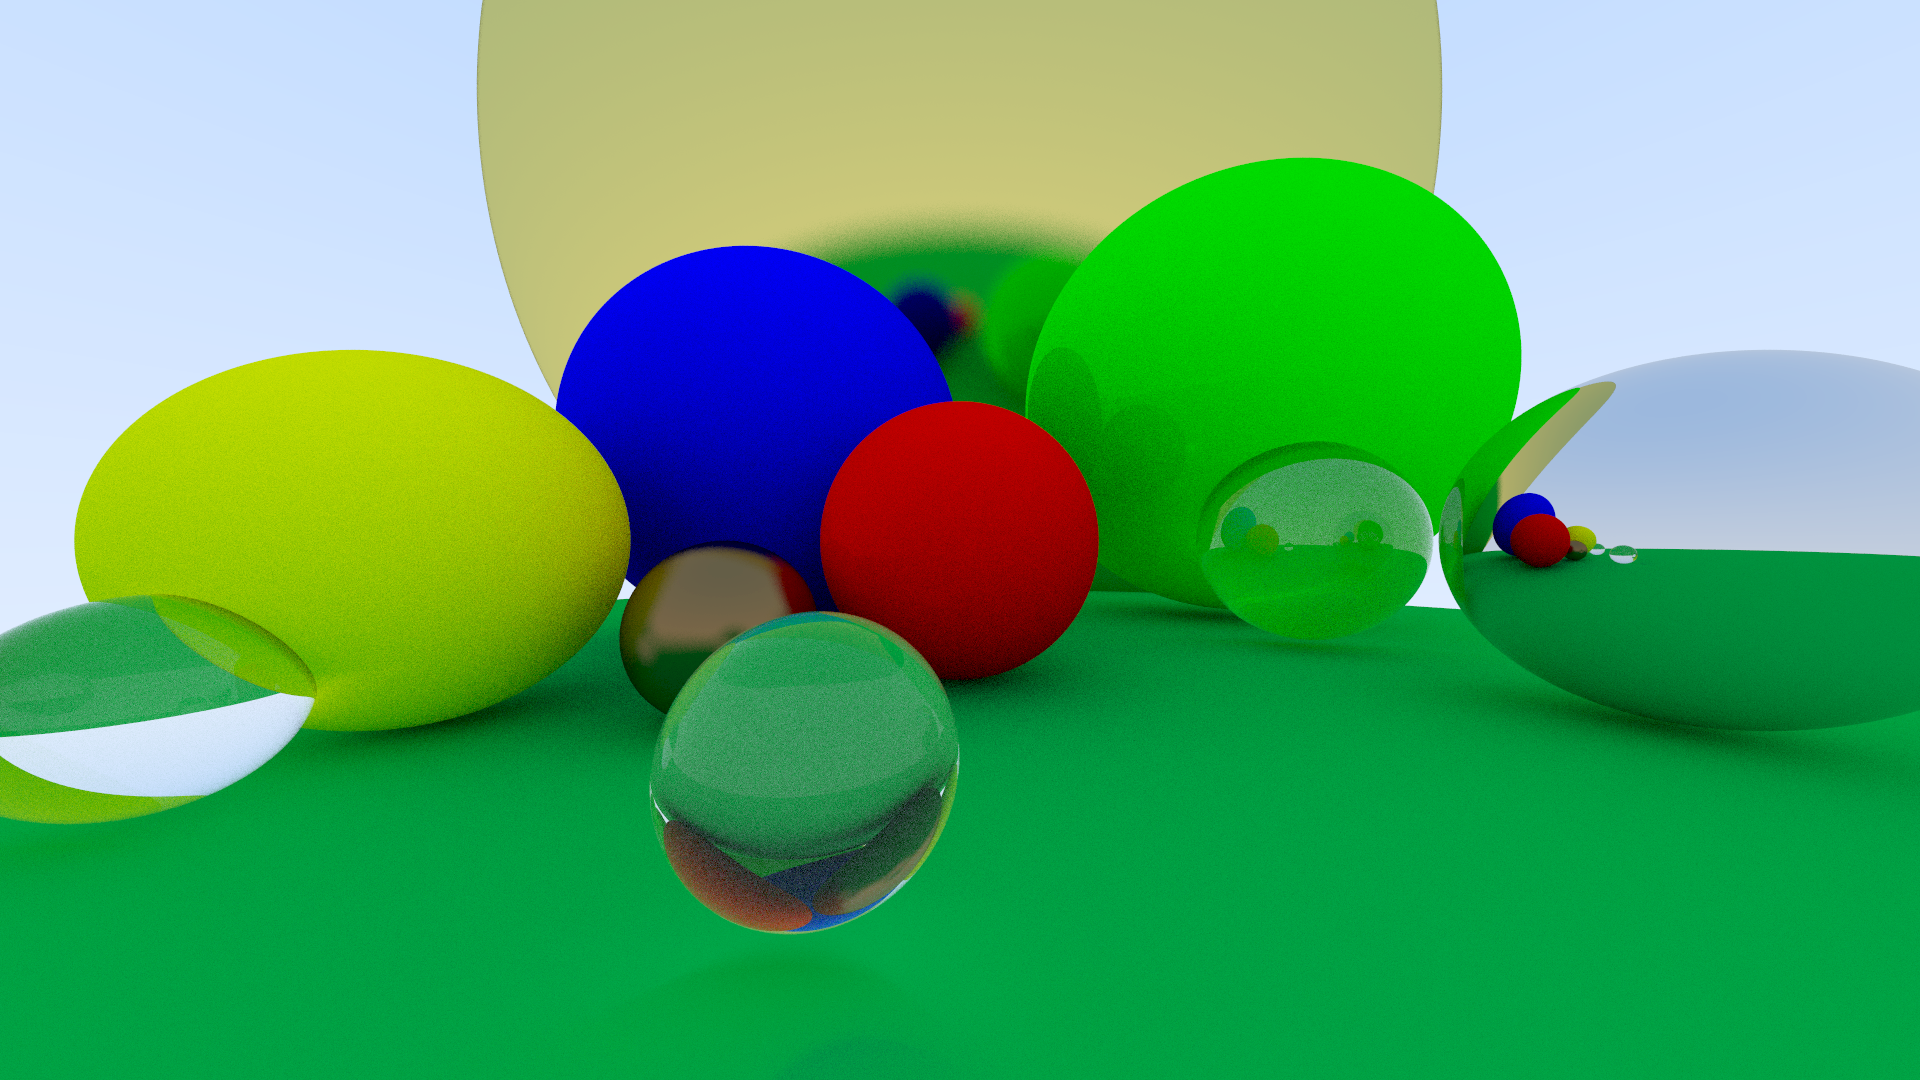
\includegraphics[width=\textwidth]{title}
\end{figure}
\begin{center}
{\Large Timo Salisch}
\end{center}
\clearpage

\tableofcontents

\newpage
\chapter{Rendering loop}
\label{chp:step1}
\pagenumbering{arabic}
The rendering process consists of two loops. One outer loop which iterates through the rows of the image and the inner loop iterating through the columns of the image. This way, every pixel will be visited once and the color of the pixel can be calculated. In this basic version of the rendering loop the color of every pixel will be set to (128, 64, 255). The resulting image can be seen in figure \ref{fig:step1}.
\begin{figure}[h!]

\includegraphics[width=\textwidth]{step1}
\centering
\caption{Result after running simple rendering loop}
\label{fig:step1}
\end{figure} \\
To store the already rendered information about the image, an \textit{Image} class is implemented. An instance of this class represents one image and saves the color information of every pixel using a two dimensional list. The color is represented as an instance of the \textit{Vector} class. This \textit{Vector} class saves three floating point values and offers simple arithmetic operations of (three-dimensional) vectors. These three values can either be interpreted as the world coordinates x, y and z or as the color properties red, green and blue. To change the color value of a specific pixel of the image, the \textit{Image} class provides an \textit{update} method to do so. In order for the image to be viewed, it has to be saved. The image is saved in the ''PPM'' format. This is done by the \textit{save\_image} method which expects a path and then saves the image to that path using the ''PPM'' format. For the file to be readable as ''PPM'', the first three lines have to include: ''P3'', image width and height, max color value. The actual pixel information are added by the loop iterating through the pixels. It is import to iterate through the rows beginning with the top row, otherwise the image is flipped. The saving process can be seen in source code \ref{lst:saving}.
\begin{lstlisting}[caption={Saving an image}, label=lst:saving, style=mystyle]
def save_image(self, path: str):
    image_str = f'P3\n{self.width} {self.height}\n255'
  
    for j in range(self.height)[::-1]:
        for i in range(self.width):
            red, green, blue = self.matrix[i][j].to_tuple()
            image_str = image_str + f"\n{int(red)} {int(green)} {int(blue)}"

    with open(path, mode='w+') as f:
        f.write(image_str)
\end{lstlisting}

\chapter{Camera}
The project is extended by a \textit{Ray} and \textit{Camera} class. A ray can be used to find all objects that need to be projected onto one pixel and thus finding the color of a pixel. Every ray has an origin and a direction, with both being instances of the \textit{Vector} class. It is possible to get the position of a ray through its method \textit{position}. The camera represents the observer of the scene and has properties such as position and information about the image. The rendering loop from chapter \ref{chp:step1} is moved into the camera class. It uses the cameras properties to find the color for every pixel. This is done by sending a ray from the camera to every pixel and finding the color of this ray. Because there are no objects in the scene yet, the color of a ray is the color of the background at that position as shown in source code \ref{lst:step2}.
\begin{lstlisting}[caption={Color of ray}, label=lst:step2, style=mystyle]
def get_color(ray: Ray):
    unit_direction = ray.direction.normalize()
    t = 0.5 * (unit_direction.y + 1)
    ray_color = Vector(255, 255, 255) * (1 - t) + Vector(127.5, 178.5, 255) * t
    return ray_color
\end{lstlisting}
This results in an image which goes from light blue at the top to a white color at the bottom, as can be seen in figure \ref{fig:step2}.
\begin{figure}[h!]

\includegraphics[width=\textwidth]{step2}
\centering
\caption{Rendering with camera and colored background}
\label{fig:step2}
\end{figure}

\chapter{Objects: shape}
After adding a camera to the scene, the next logical step is to add objects. The chosen object to start with are spheres. For this a class \textit{Sphere} is implemented, which takes a vector as origin, a radius and a color vector. A \textit{Sphere} instance can return if a given ray hits it and if so, can calculate the intersection point of the ray and itself and its normal vector at that point. The normal vector is chosen to always point outwards of the sphere. If a ray hits a sphere, the ray adopts the color of the sphere. To better organize the handling of the sphere objects, a \textit{Scene} class is used. This class represents the scene and holds the camera and all objects in this scene. The objects are stored in an instance of the \textit{World} class. This class is basically an abstracted list with the benefit, that it provides a \textit{hit} method. Like the equivalent method of the \textit{Sphere} class, it determines if the ray hits an object. But this method checks all spheres and returns the information about the sphere, that gets hit by the ray first. This solves the visibility problem of multiple spheres being stacked behind each other. It also simplifies the rendering loop to not having to iterate through all spheres, because this is done internally by this method. To keep the interface simple, the \textit{Scene} class also offers a \textit{render} method which just forwards to the equivalent method of the camera. This way, all required actions can be performed using a \textit{Scene} instance which, after rendering, returns an \textit{Image} instance that can be used as needed. To change the scene after creation, it provides a function to add spheres to it. This class structure simplifies the whole process from creating to rendering and saving the image to:
\begin{itemize}
\item Creating a \textit{Camera} instance with preferred properties
\item Creating a \textit{Scene} object giving the camera instance as a parameter
\item Creating and adding as many \textit{Sphere} instances to the scene object as wanted
\item Using \textit{render} function of scene
\item Saving resulted \textit{Image} object to any path
\end{itemize}
Using this procedure, images can be created that contain multiple spheres. Every sphere can have a different color, position and size. If at a position in the image there is no sphere, the background color introduces in the previous chapter is kept. At this point the created rendered has solved the visibility problem, even though in a pretty simple setting. An example of an image created by this renderer is displayed in figure \ref{fig:step3}.
\begin{figure}[h!]
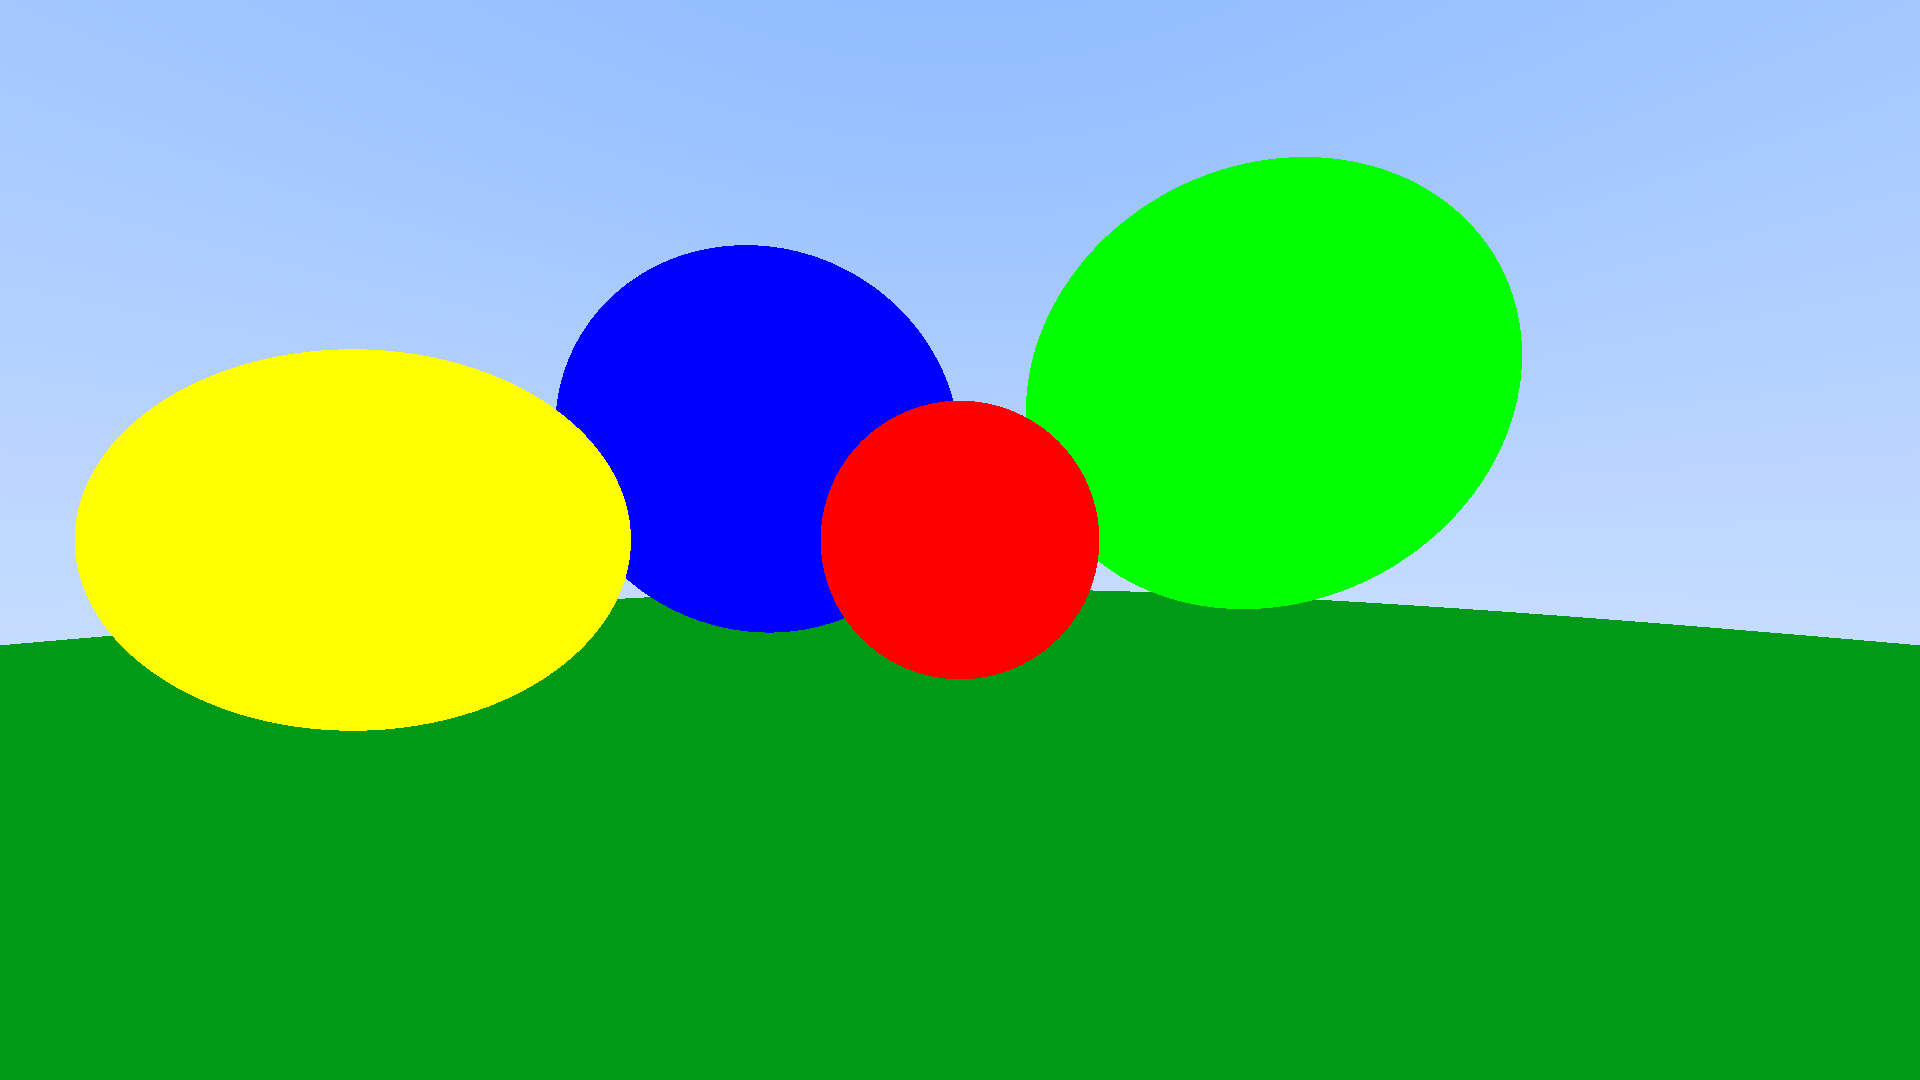
\includegraphics[width=\textwidth]{step3}
\centering
\caption{Image created by simple renderer}
\label{fig:step3}
\end{figure}

\chapter{Enhancing camera and rendering loop}
On the rendered images the spheres seem round, but this is not the actually the case. They only look round because of the ''high'' quality and thus the pixels being pretty small. By zooming into the image at the border of a sphere this can be seen more clearly (figure \ref{fig:aliasing}).
\begin{figure}[h!]

\includegraphics[width=\textwidth]{aliasing}
\centering
\caption{Zoomed in sphere border}
\label{fig:aliasing}
\end{figure} \\
The reason for this is, that only one ray is sent through each pixel at the left end of the pixel. With spheres being round in reality but monitors only being able to display things using pixels, this is no unexpected behavior. But if pixels are bigger -- either because of a lower resolution or because the images are shown on a bigger screen -- this can make the image look unnatural and wrong. One way of improving the border would be using colors in between the two colors (here red and green). This would make the edge less harsh and thus the sphere looks more round. To keep the correct shape of the objects and not adding any visual bumps to it, the color has to be mixed of the two colors keeping the ratio of the objects in this pixel into account. To not having to calculate the ratio for every pixel, which is computational expensive, multiple rays are sent through each pixel at random positions of the pixel. The average color of these rays can then be used as the color of the pixel. The more rays are used per pixel, the closer will the average color be to the true color.
\begin{figure}[h!]
\centering
\begin{subfigure}[h!]{0.475\textwidth}
\centering

\includegraphics[width=\textwidth]{step4_2rays}
\caption{2 rays per pixel}
\end{subfigure}
\hfill
\begin{subfigure}[h!]{0.475\textwidth}
\centering

\includegraphics[width=\textwidth]{step4_4rays}
\caption{4 rays per pixel}
\end{subfigure}
\vskip\baselineskip
\begin{subfigure}[h!]{0.475\textwidth}
\centering

\includegraphics[width=\textwidth]{step4_8rays}
\caption{8 rays per pixel}
\end{subfigure}
\hfill
\begin{subfigure}[h!]{0.475\textwidth}
\centering

\includegraphics[width=\textwidth]{step4_16rays}
\caption{16 rays per pixel}
\end{subfigure}
\caption{Zoomed in sphere border with a different number of rays per pixel}
\label{fig:step4}
\end{figure} \\
From figure \ref{fig:step4} can be seen, that the more rays are used per pixel the more different color shades are used at the sphere's border. In comparison to only one ray (figure \ref{fig:aliasing}), it is visible that the sphere's edge becomes much smoother the more rays are used.

\chapter{Objects material: diffuse}
The images produced so far look rather 2D than 3D, it seems like there is no depth in the image. This is caused by the uniform color of the spheres. In the real world, a sphere has reflections on it and the color looks different depending of the viewing angle. Also there are no shadows of the spheres on one another if they are close. To solve this and make the image more realistic, materials are introduced. A parent class \textit{Material} defines all methods needed for a material. Instead of a color, every sphere now gets a material that contains the color information. To make the rendered backwards compatible and being able to still recreate previous images, a \textit{NoTexture} material is implemented. This material has no texture and only has its color, simulating the appearance of spheres without materials. By doing so, a consisting interface is created where every sphere has a material and the methods provided by the \textit{Material} can always be used. Therefore, \textit{NoTexture} and all other implemented materials inherit from the \textit{Material} class. To have a simple texture for the spheres, the material \textit{Diffuse} is added. This reflects the ray, when hit by it, in a random direction following it normal vector at this point. By using the normal vector as the baseline for the reflected ray, the curvature of the sphere becomes visible. But to make it more realistic, a bit of randomness is added on top of the normal vector. The ray now does simply takes the color of the sphere it has hit, but  follows in the reflected direction to see if it hits another object there. This way, the ray that, in the normal world would come from the light source, bounce of some objects and then go into the camera, is simulated backwards. At this point, the only source of light is the background. By modulating all colors the ray encounters on its way, the final color can be determined. It is done in a way where the color components are multiplied with each other. This is realistic taking into account that complementary colors if mixed result in black in the real world and also with this modulation. The modulation is shown in source code \ref{lst:modulation}. \\\\\\
\begin{lstlisting}[caption={Modulating two colors}, label=lst:modulation, style=mystyle]
def modulate(self, other: Vector) -> Vector:
    return Vector(self.x * other.x / 255, self.y * other.y / 255, self.z * other.z / 255)
\end{lstlisting}
Because the program needs to be terminated at some point, a maximum number of times the ray can bounce of objects has to be defined. Otherwise it could occur, that the ray gets stuck between multiple objects always going from one object to the other and the program therefore never finishing. If this maximum number of bounces is reached, the color of the ray is set to black, because it did not come from a light source. The influence of the render depth (the maximum number of bounces) onto the finale image can be seen in figure \ref{fig:step5}. It can be seen, that the bigger the render depth the less noise the image appears. In the real world the light ray can bounce of unlimited time (assuming the light does not lose energy by absorption or scattering). With a higher render depth, it is more likely that the light source of the ray is found and thus the ray does not get set to black. These ''false'' black rays happen more often with a lower render depth letting the image seem noisy. A render depth of 1 is the extreme case of this, here every ray that hits an object is assumed to not come from a light source portraying all spheres as black. \\
Simply modulating as shown in source code \ref{lst:modulation} causes the rays to become darker the more often they are reflected. Because of that the image is getting darker which is not wanted. To reduce this effect, the image needs to be gamma corrected. This is done by taking the square root of the relative intensity of the color component (hence the color component in an interval of 0 to 1). The gamma correction is represented in source code \ref{lst:gamma}.
\begin{lstlisting}[caption={Gamma correction}, label=lst:gamma, style=mystyle]
red = math.sqrt(red / 255) * 255
green = math.sqrt(green / 255) * 255
blue = math.sqrt(blue / 255) * 255
\end{lstlisting}
\begin{figure}[h!]
\centering
\begin{subfigure}[h!]{0.475\textwidth}
\centering
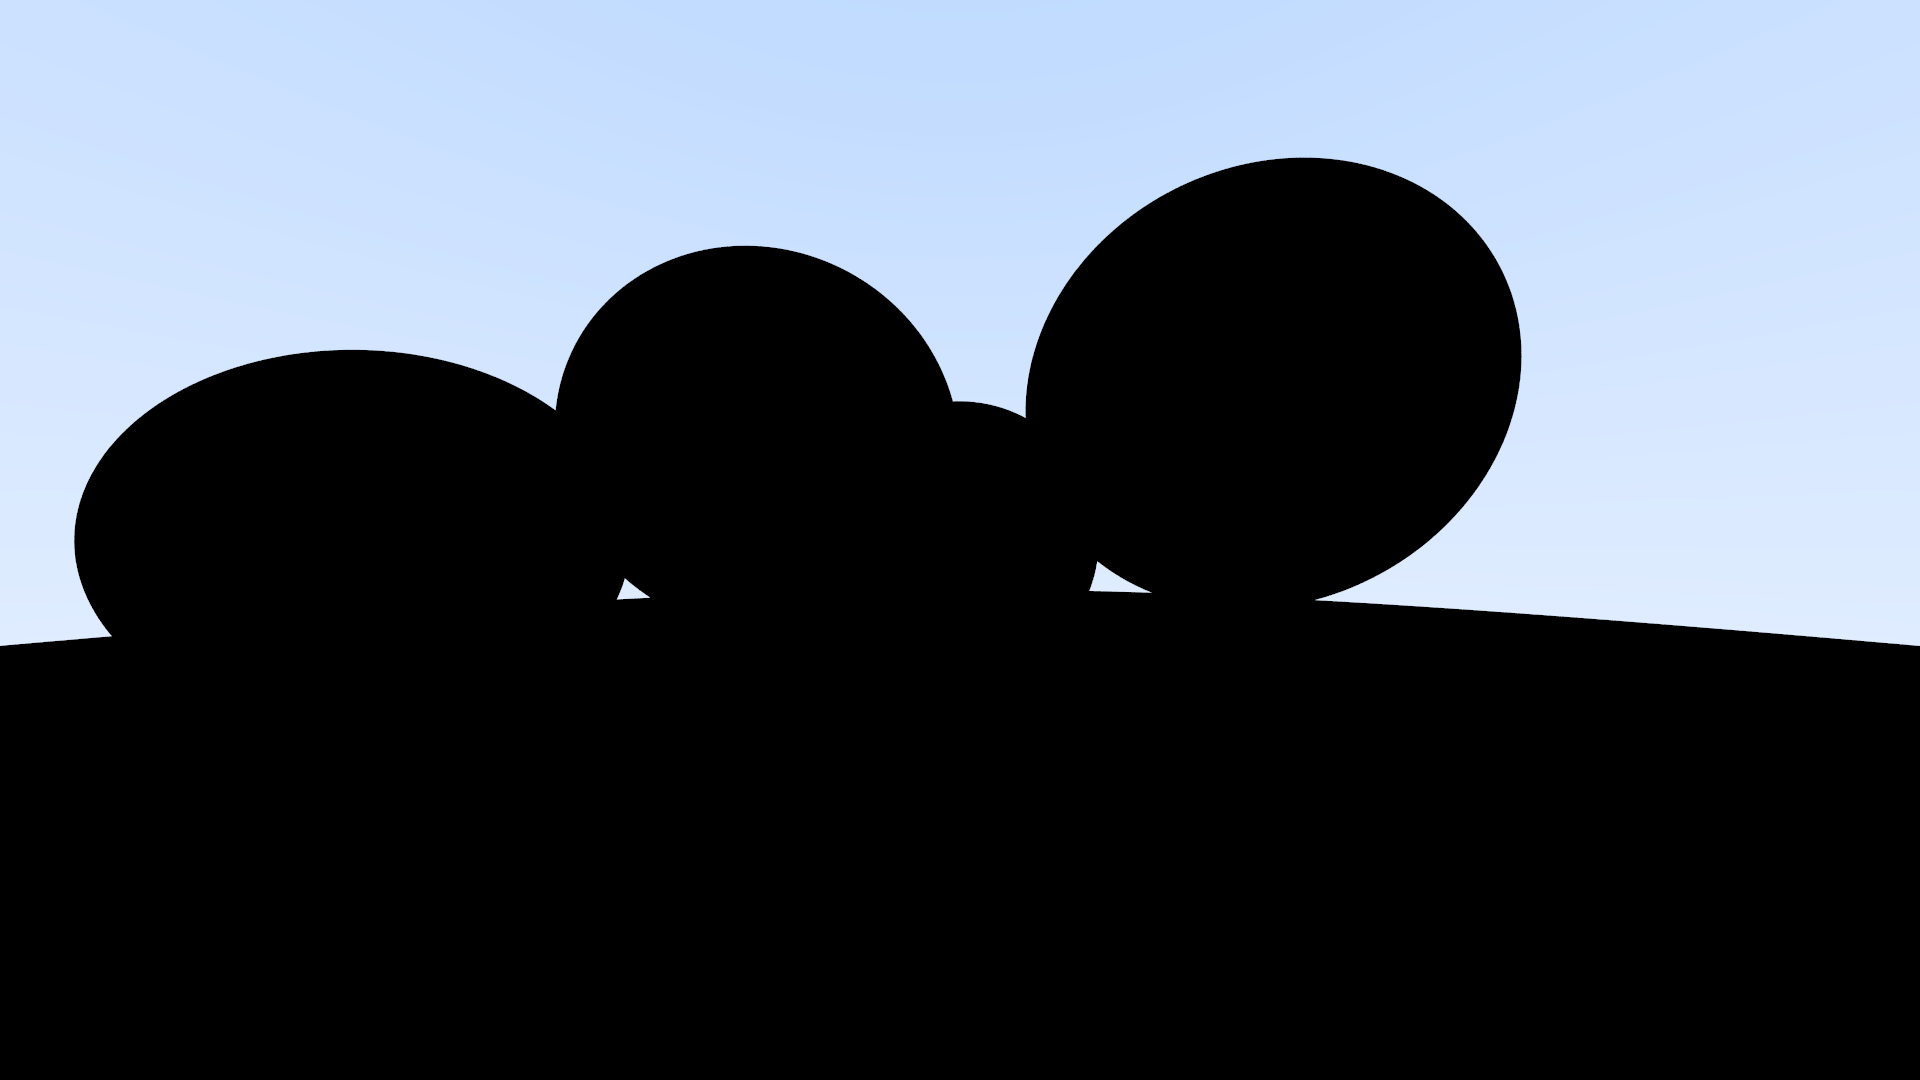
\includegraphics[width=\textwidth]{step5_depth1}
\caption{Render depth 1}
\end{subfigure}
\hfill
\begin{subfigure}[h!]{0.475\textwidth}
\centering
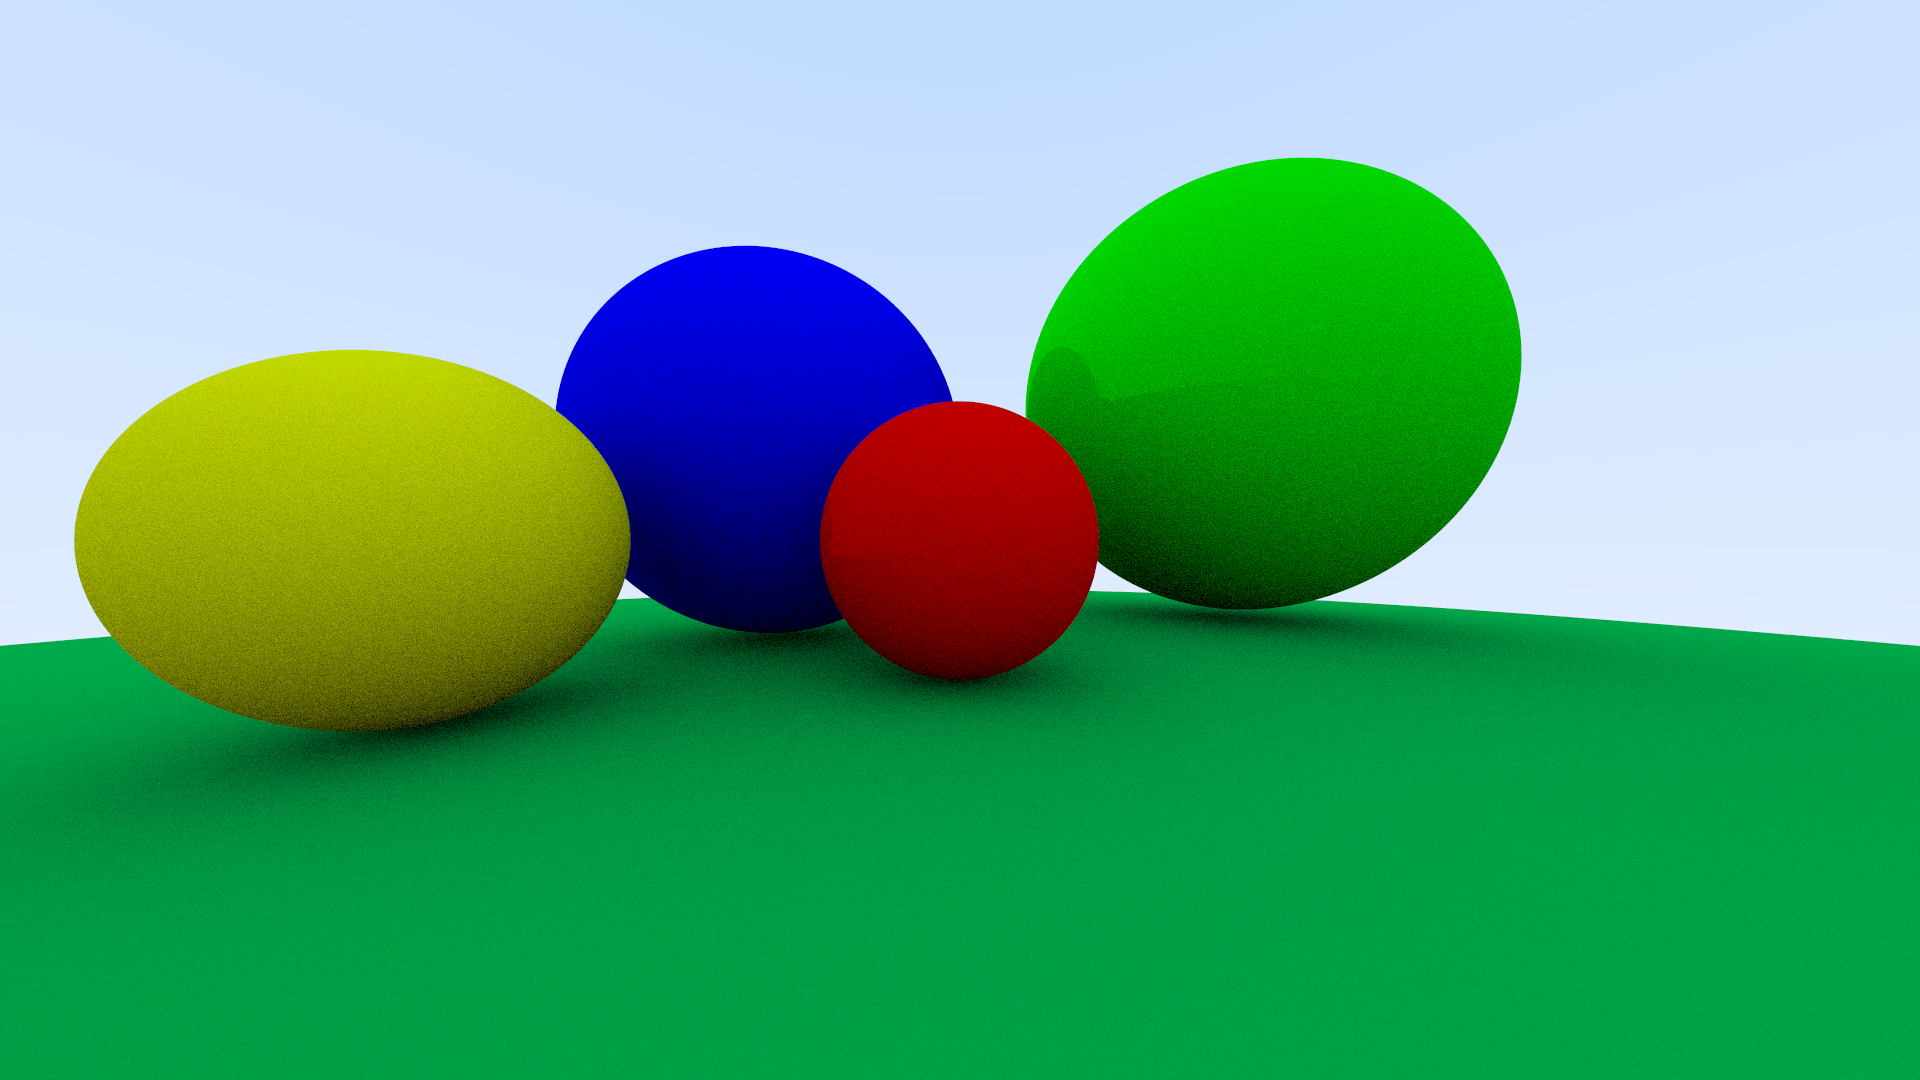
\includegraphics[width=\textwidth]{step5_depth2}
\caption{Render depth 2}
\end{subfigure}
\vskip\baselineskip
\begin{subfigure}[h!]{0.475\textwidth}
\centering
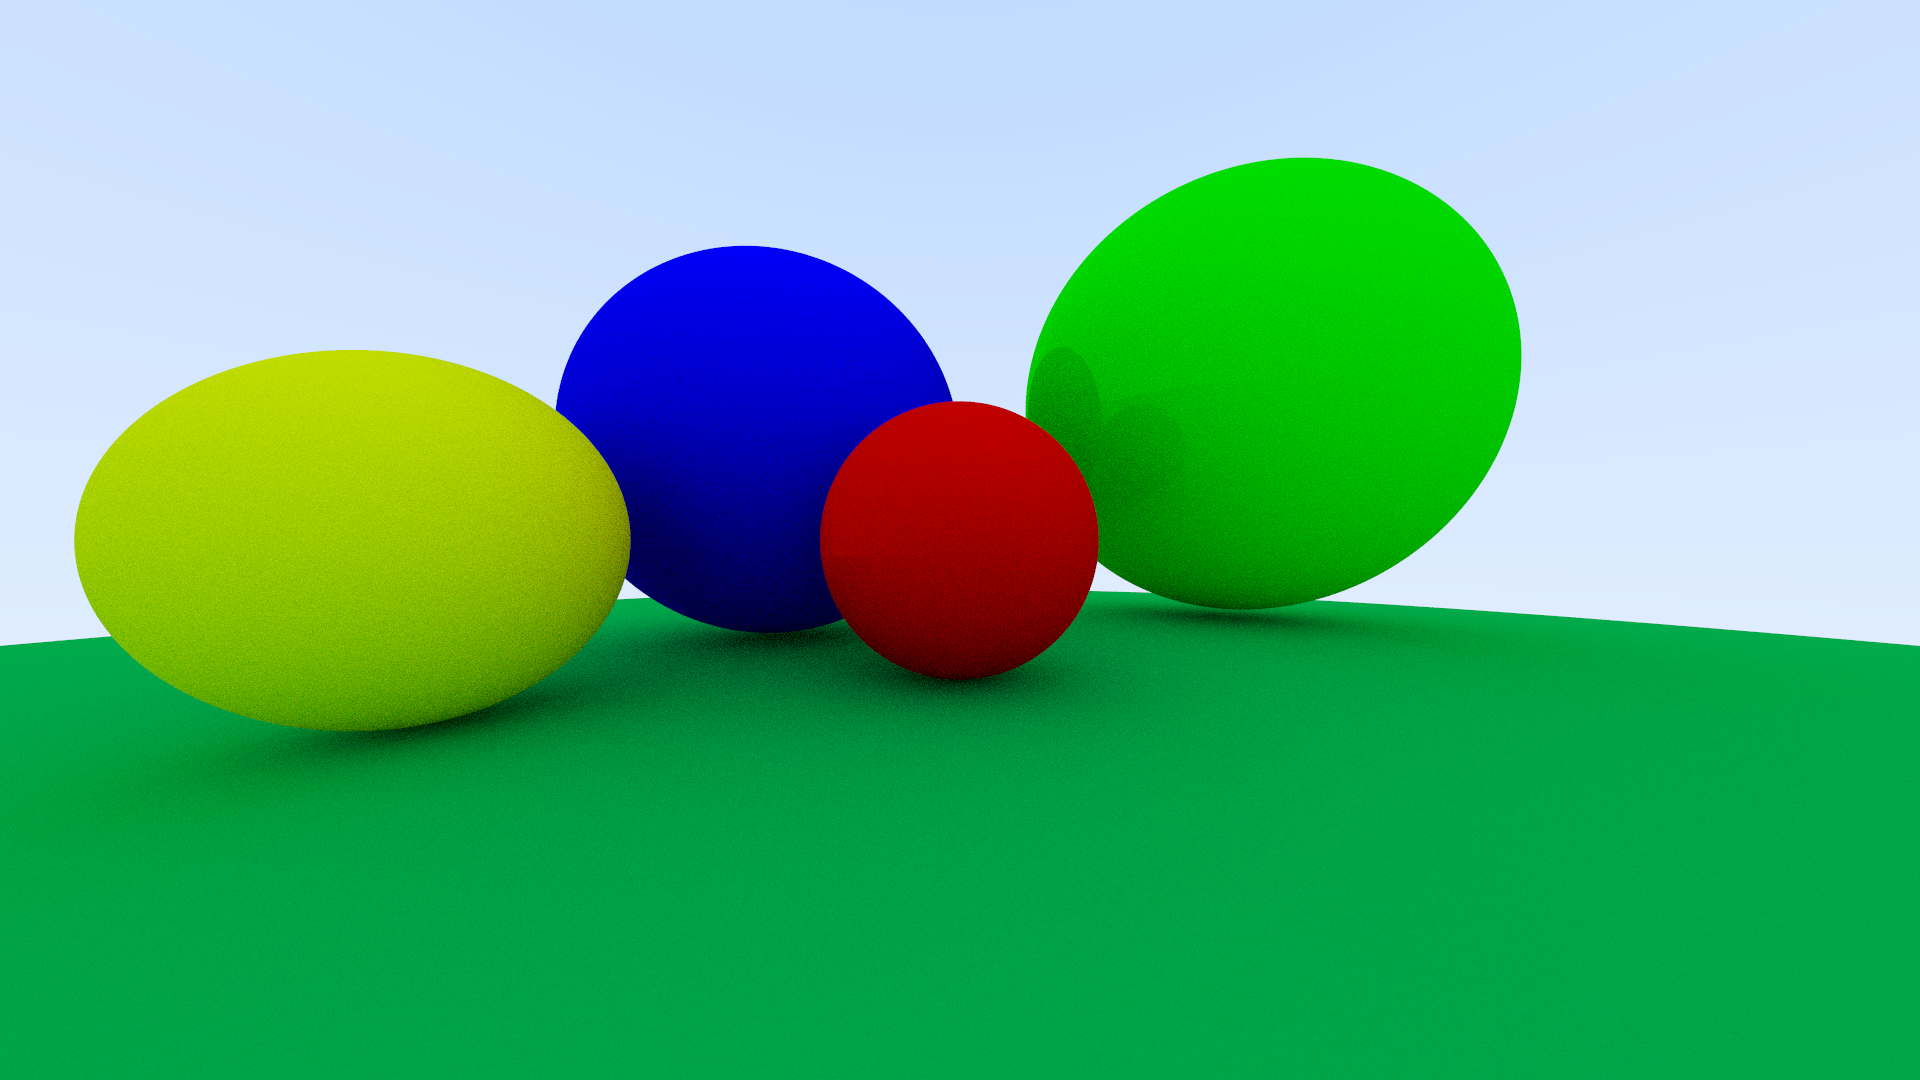
\includegraphics[width=\textwidth]{step5_depth4}
\caption{Render depth 4}
\end{subfigure}
\hfill
\begin{subfigure}[h!]{0.475\textwidth}
\centering
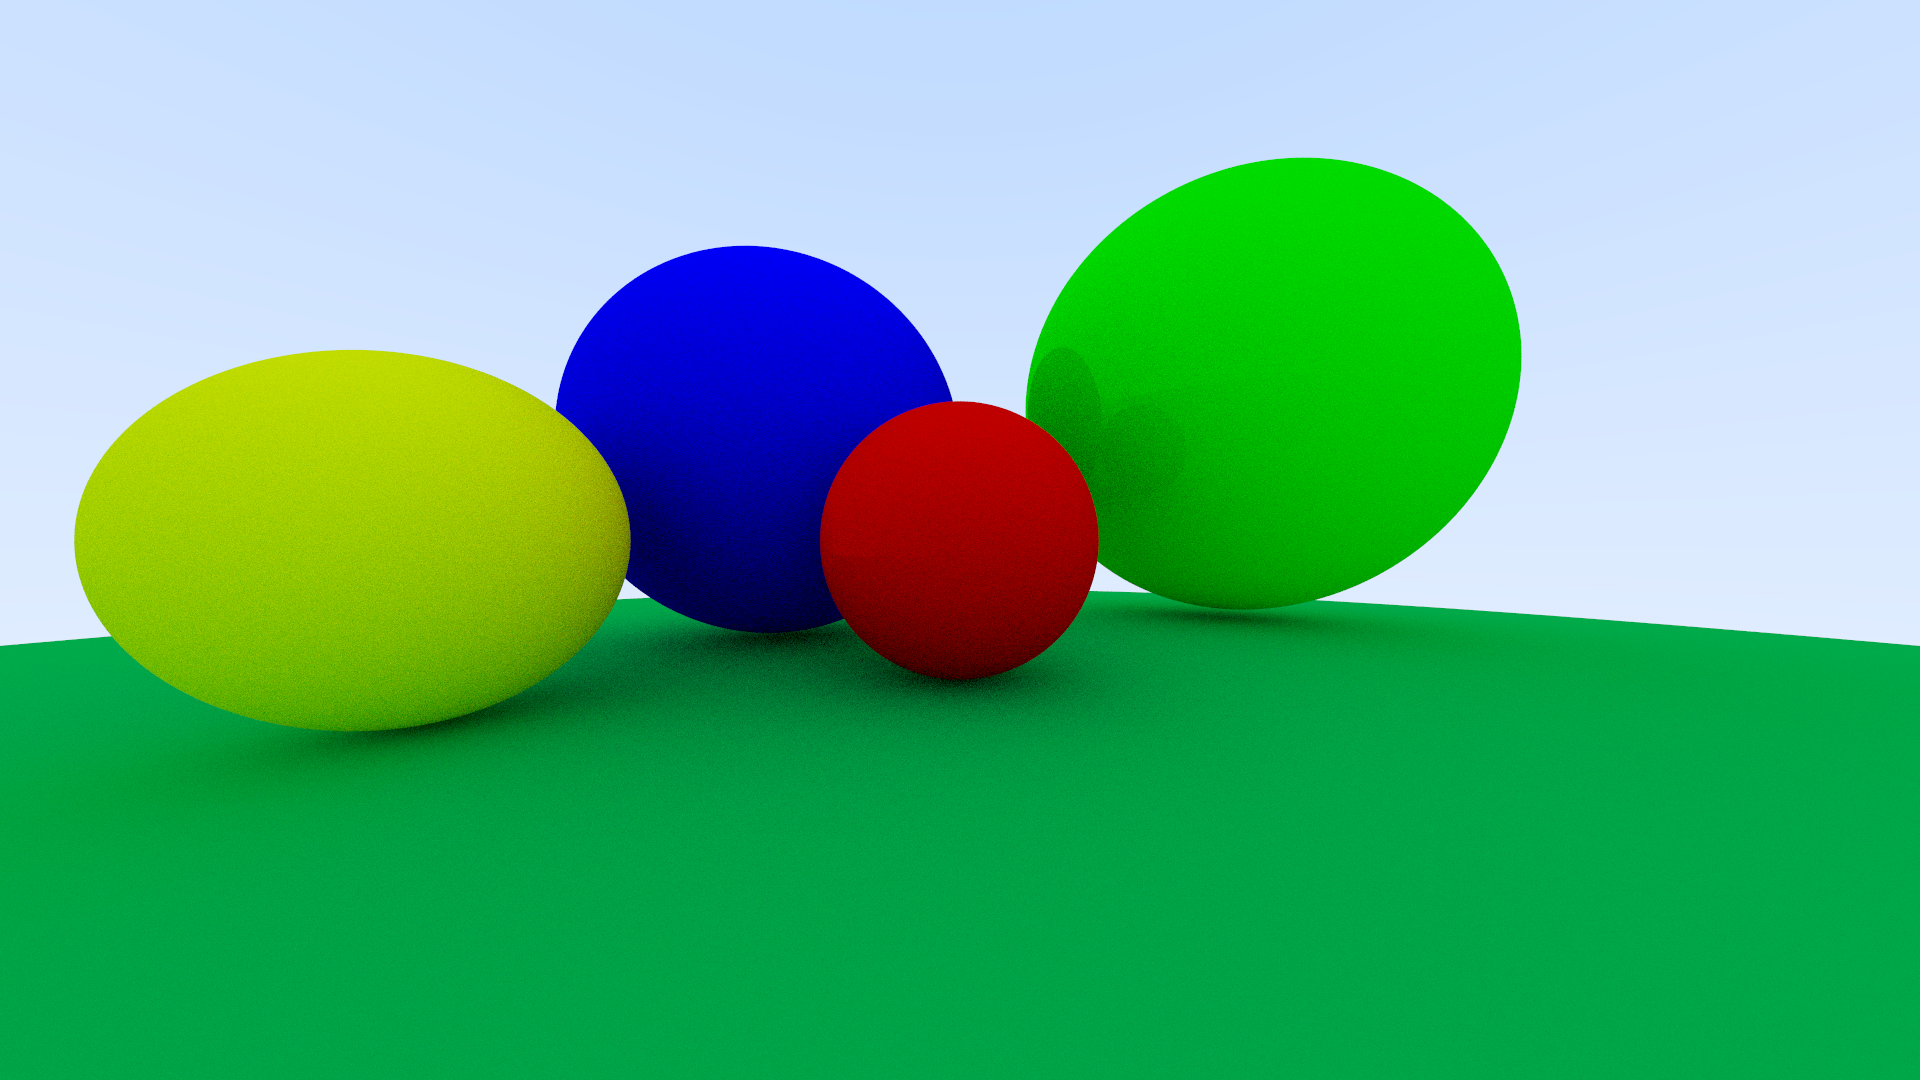
\includegraphics[width=\textwidth]{step5_depth8}
\caption{Render depth 8}
\end{subfigure}
\vskip\baselineskip
\begin{subfigure}[h!]{0.475\textwidth}
\centering
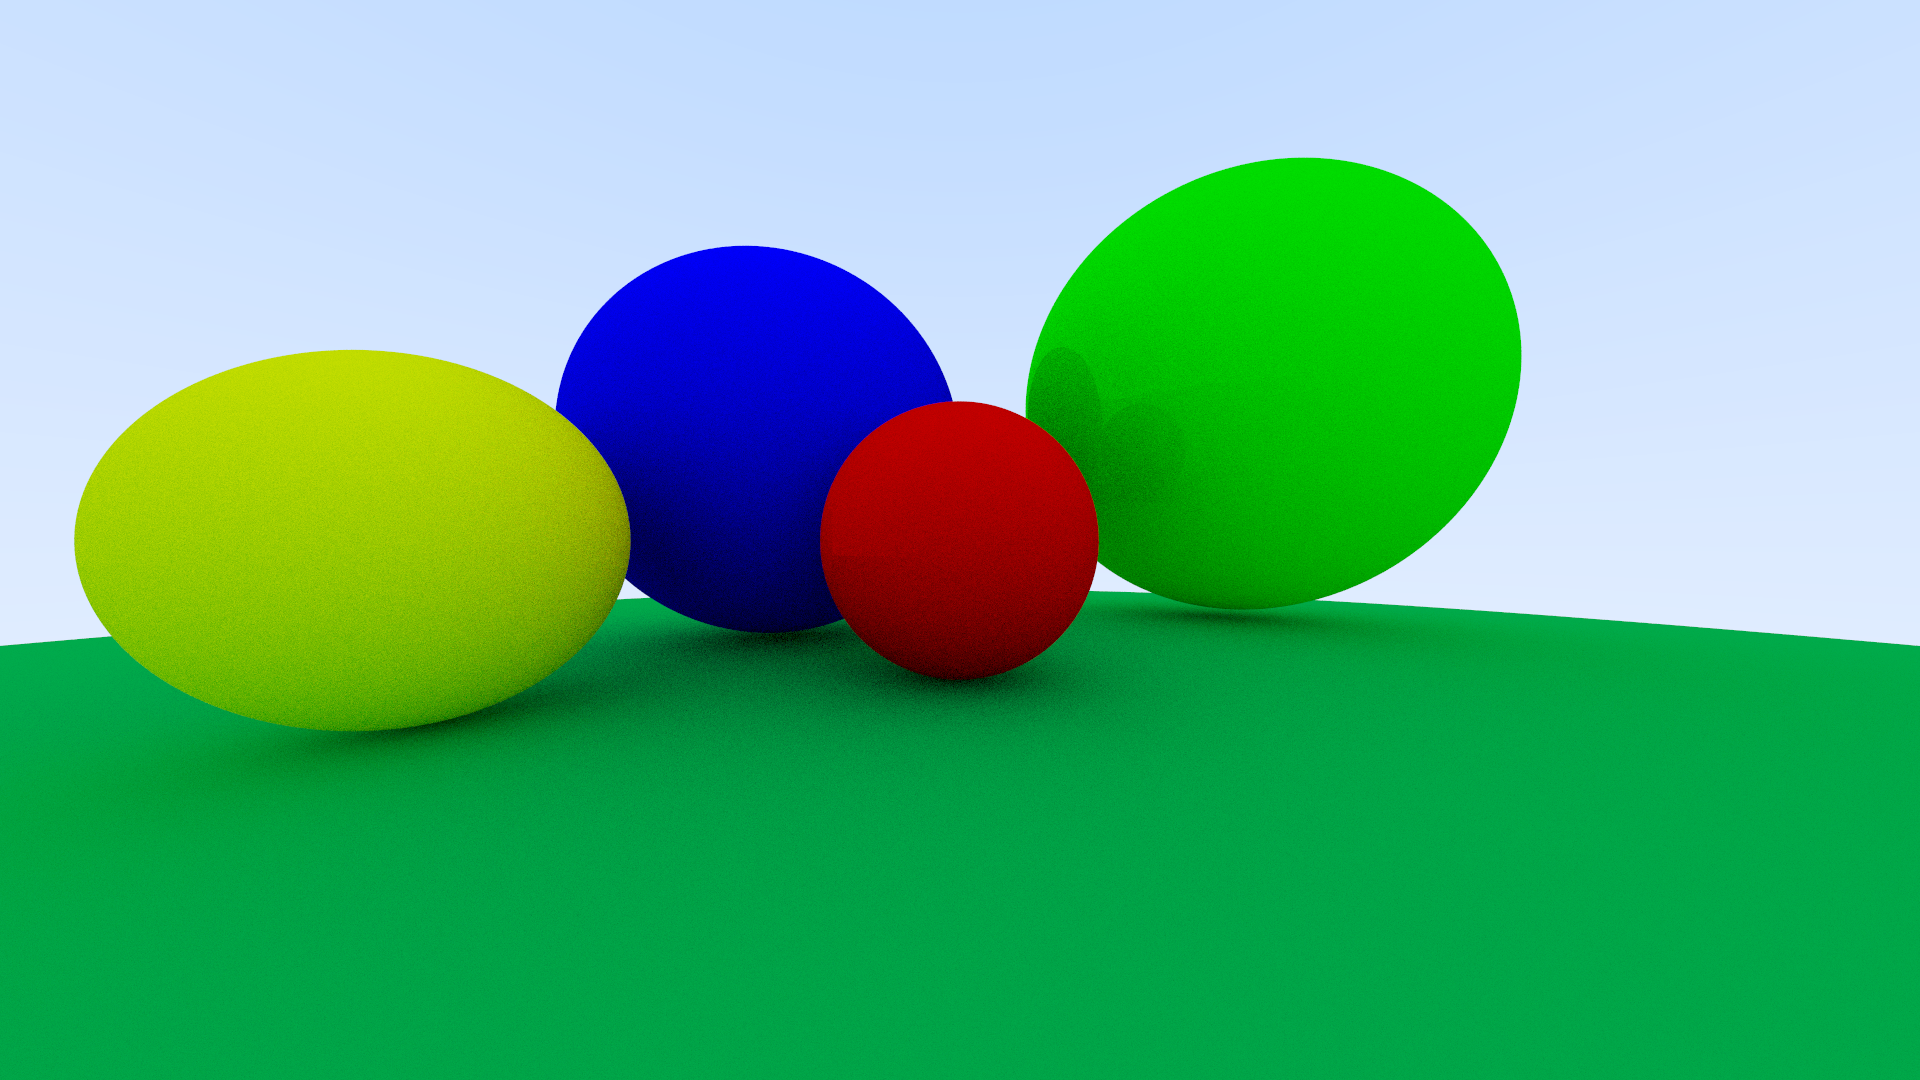
\includegraphics[width=\textwidth]{step5_depth16}
\caption{Render depth 16}
\end{subfigure}
\caption{Spheres with diffuse material and different render depths}
\label{fig:step5}
\end{figure}

\chapter{Objects material: specular}
The next material introduced into the image is specular. This material reflects the rays not in a random direction but with the same angle the ray hits the sphere. Using this material, metal spheres and other reflective objects can be produced. By letting the class \textit{Specular} inherit from \textit{Material}, it can be used without changing any existing classes. To make the material more diverse, a parameter ''fuzz'' is given to it. This defines the clearness of the material, 0 being perfectly reflective and the higher the number the less clear the reflection gets. It is achieved by adding a random component to the reflected ray. If ''fuzz'' is 0, no randomness is added to the reflected ray and the bigger the ''fuzz'' the more randomness is added. Figure \ref{fig:step6} contains three spheres with specular material, the silver sphere has a ''fuzz'' of 0, the bronze 0.25 and the gold sphere a ''fuzz'' of 0.1. This shows the influence of the ''fuzz'' onto the reflected image on the sphere's surface. \\
The calculation of the reflected ray is only dependent on the normalized direction of the ray and the normal vector of the sphere at the point of intersection. The calculation is shown by source code \ref{lst:reflection}.
\begin{lstlisting}[caption={Calculating reflected ray}, label=lst:reflection, style=mystyle]
def reflect(direction: Vector, normal_vector: Vector) -> Vector:
    return direction - normal_vector * (direction * normal_vector) * 2
\end{lstlisting}
\begin{figure}[h!]
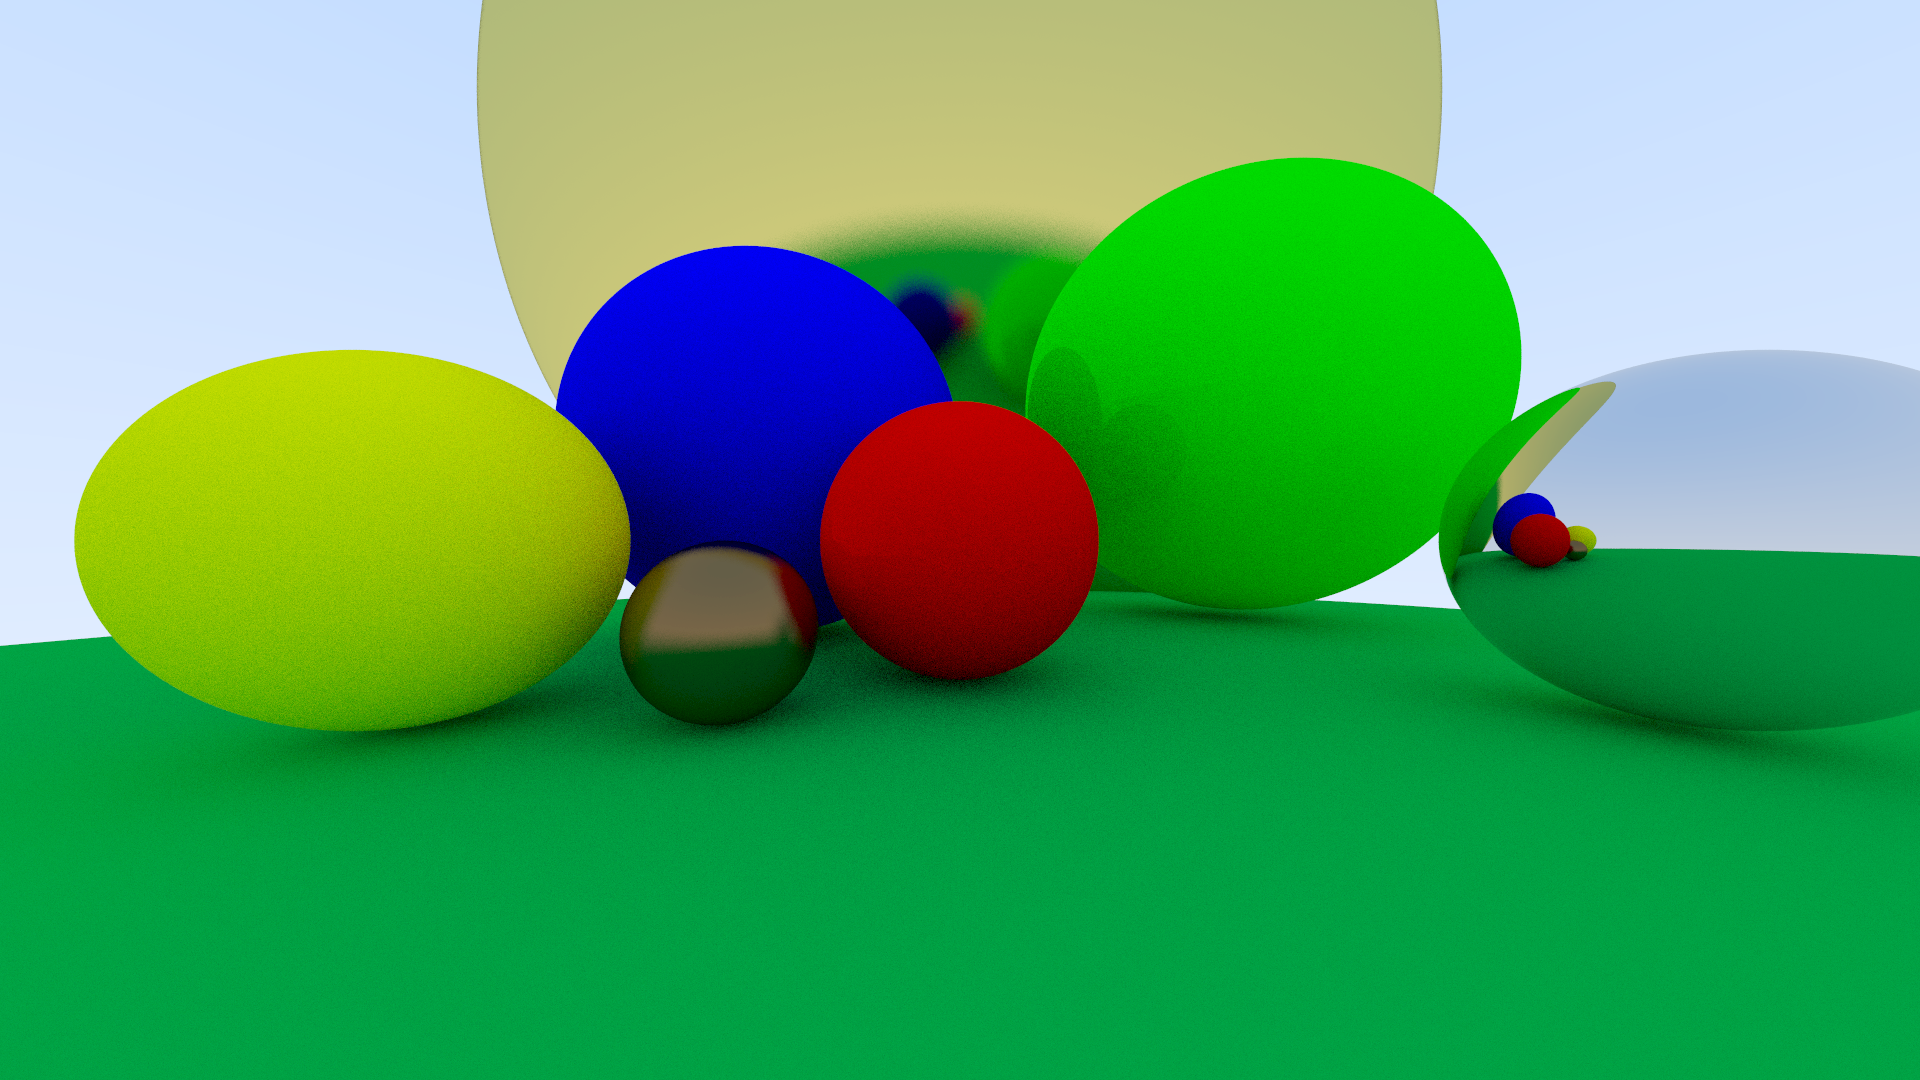
\includegraphics[width=\textwidth]{step6}
\centering
\caption{Image containing spheres with specular material (render depth 16)}
\label{fig:step6}
\end{figure}

\chapter{Objects material: specular transmission}
\vspace*{-0.1cm}
So far, all materials only reflect the rays. The next material that is added to the project is transmissive, meaning it can let rays go through the object. This characteristic is known from objects made of for example glass or diamond. By letting rays pass through the object, spheres that are behind this object are also visible through the object. Because all objects in the scene are spheres, the area behind the transmissive sphere appears flipped which is a characteristic of transmissive spheres. The transmissive spheres in figure \ref{fig:step7} demonstrate this behavior. As with all other materials, \textit{Transmissive} is a child class of \textit{Material}. These transmissive spheres also show that they not only let rays through, but also reflect some of the rays. This mix of reflected objects on its surface and objects from behind it gives the transmissive spheres its 3D appearance and let them appear more realistic. Especially towards the edge of the visible part these spheres have to mainly reflect than letting the rays pass. This is because the angle of the rays are too steep to enter the spheres. To calculate which rays are reflected, the Schlick Approximation is used. This is a computational efficient way of solving this problem while still producing realistic results. To determine the direction of the passing rays, the function shown in source code \ref{lst:refraction} is used.
\begin{lstlisting}[caption={Calculating refracted ray}, label=lst:refraction, style=mystyle]
def refract(direction: Vector, normal_vector: Vector, refraction_ratio: float, factor: int) -> Vector:
    cos_theta = min(direction * normal_vector * -1 * factor, 1)
    ray_perp = (direction + normal_vector * cos_theta * factor) * refraction_ratio
    ray_parl = normal_vector * -math.sqrt(math.fabs(1 - ray_perp.length() ** 2)) * factor
    return ray_perp + ray_parl
\end{lstlisting}
The calculation is based on Snell's Law. But because it assumes that the normal vector is in the opposite direction than the ray, the signs have to be changed if they are in the same direction. The normal vector given by the spheres is always directed away from the sphere's center and thus both cases can occur, depending on if the ray wants to enter or exit the sphere. To change the signs in the equation without using if clauses, the parameter ''factor'' is introduced. This is either 1 or -1, depending on if the signs have to be inverted. The ''refraction\_ratio'' is defined by the material and is used to simulate the different refractional behaviors of real world materials such as glass and diamond.
\begin{figure}[h!]
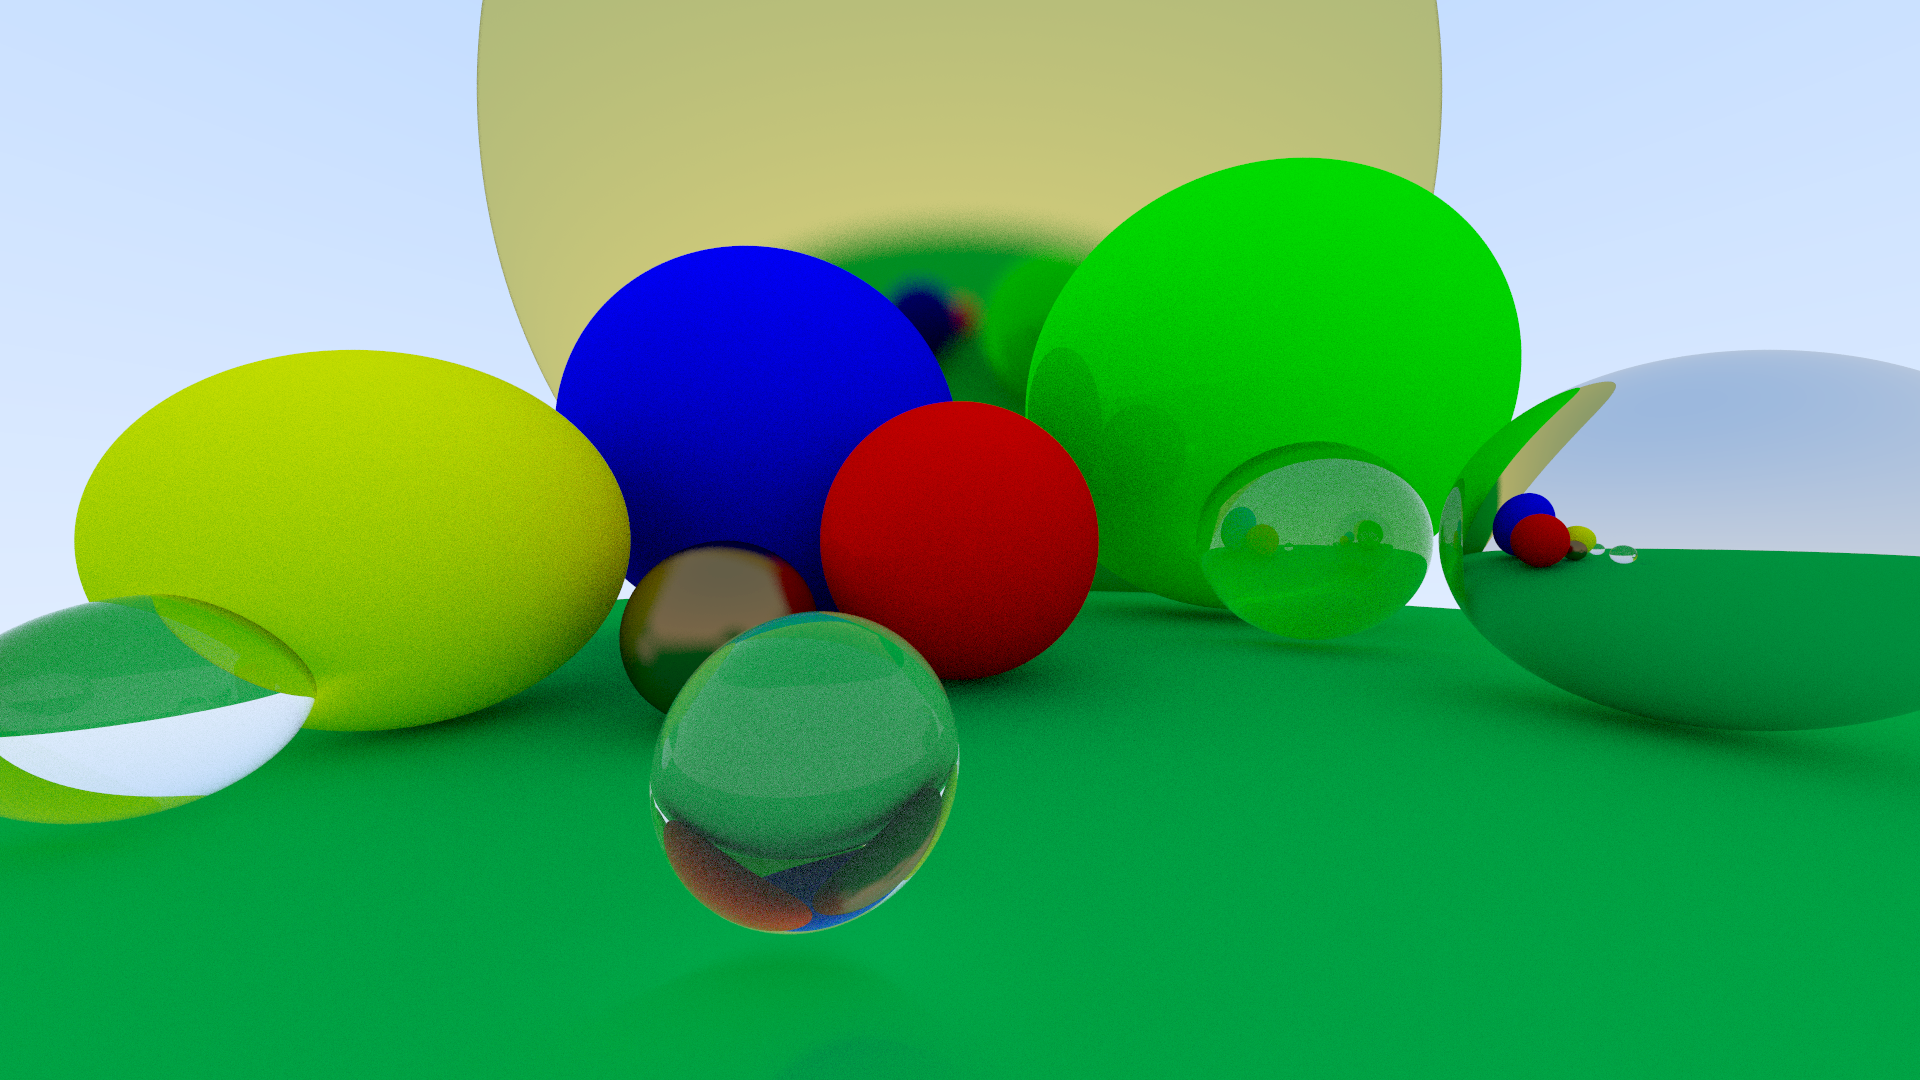
\includegraphics[width=\textwidth]{step7}
\centering
\caption{Image with added transmissive spheres (render depth 16)}
\label{fig:step7}
\end{figure}

\chapter{Lights}
So far all light is emitted by the background. To make objects emit light, a new material \textit{Emissive} has to be implemented. This has, besides it color, also a parameter defining its intensity. The lower the intensity the darker the emitted light. The emissive behavior of a material can be used by its function ''emit'', which returns the products of its color and intensity. As usual, the class \textit{Emissive} inherits from \textit{Material}. To not have to differentiate between emissive and non-emissive materials, the interface of the \textit{Material} class is also extended by the method ''emit''. If not overwritten by a child class, this method returns simply no light (black). Hence the same source code can be used once again for all materials not having to differentiate between different materials but now including light emitting objects. The value of the emitted light is simply added to the color of the hitting ray. To give emitting objects more importance, the color of the background has be changeable. This is achieved by defining a background color that is returned if a ray does not hit an object (mostly chosen to be black which is equivalent to no light emitted from the background). To still recreate previous images, the same background is used as before if no background color is defined. Figure \ref{fig:step8} shows the influence of emitting objects without a background light onto the image from \ref{fig:step7}. It can be seen that if parts of a sphere's surface are not hit by any light they stay black (visible on the big gold sphere in the center). Now every ray, starting from the camera and hitting an object, needs to hit an emissive object in the end to not be black. So if all light emitting spheres rather small, the whole image will be pretty dark. To avoid that, the slightly visible big sphere above all other spheres is gigantic so that the scene is bright enough. If the space would be enclosed by objects so that the light gets reflected to all places, a smaller light source is sufficient for a similar brightness. To further not distort the spheres colors, a white light sources should be chosen, otherwise all objects will seem as if they have a different color.
\begin{figure}[h!]
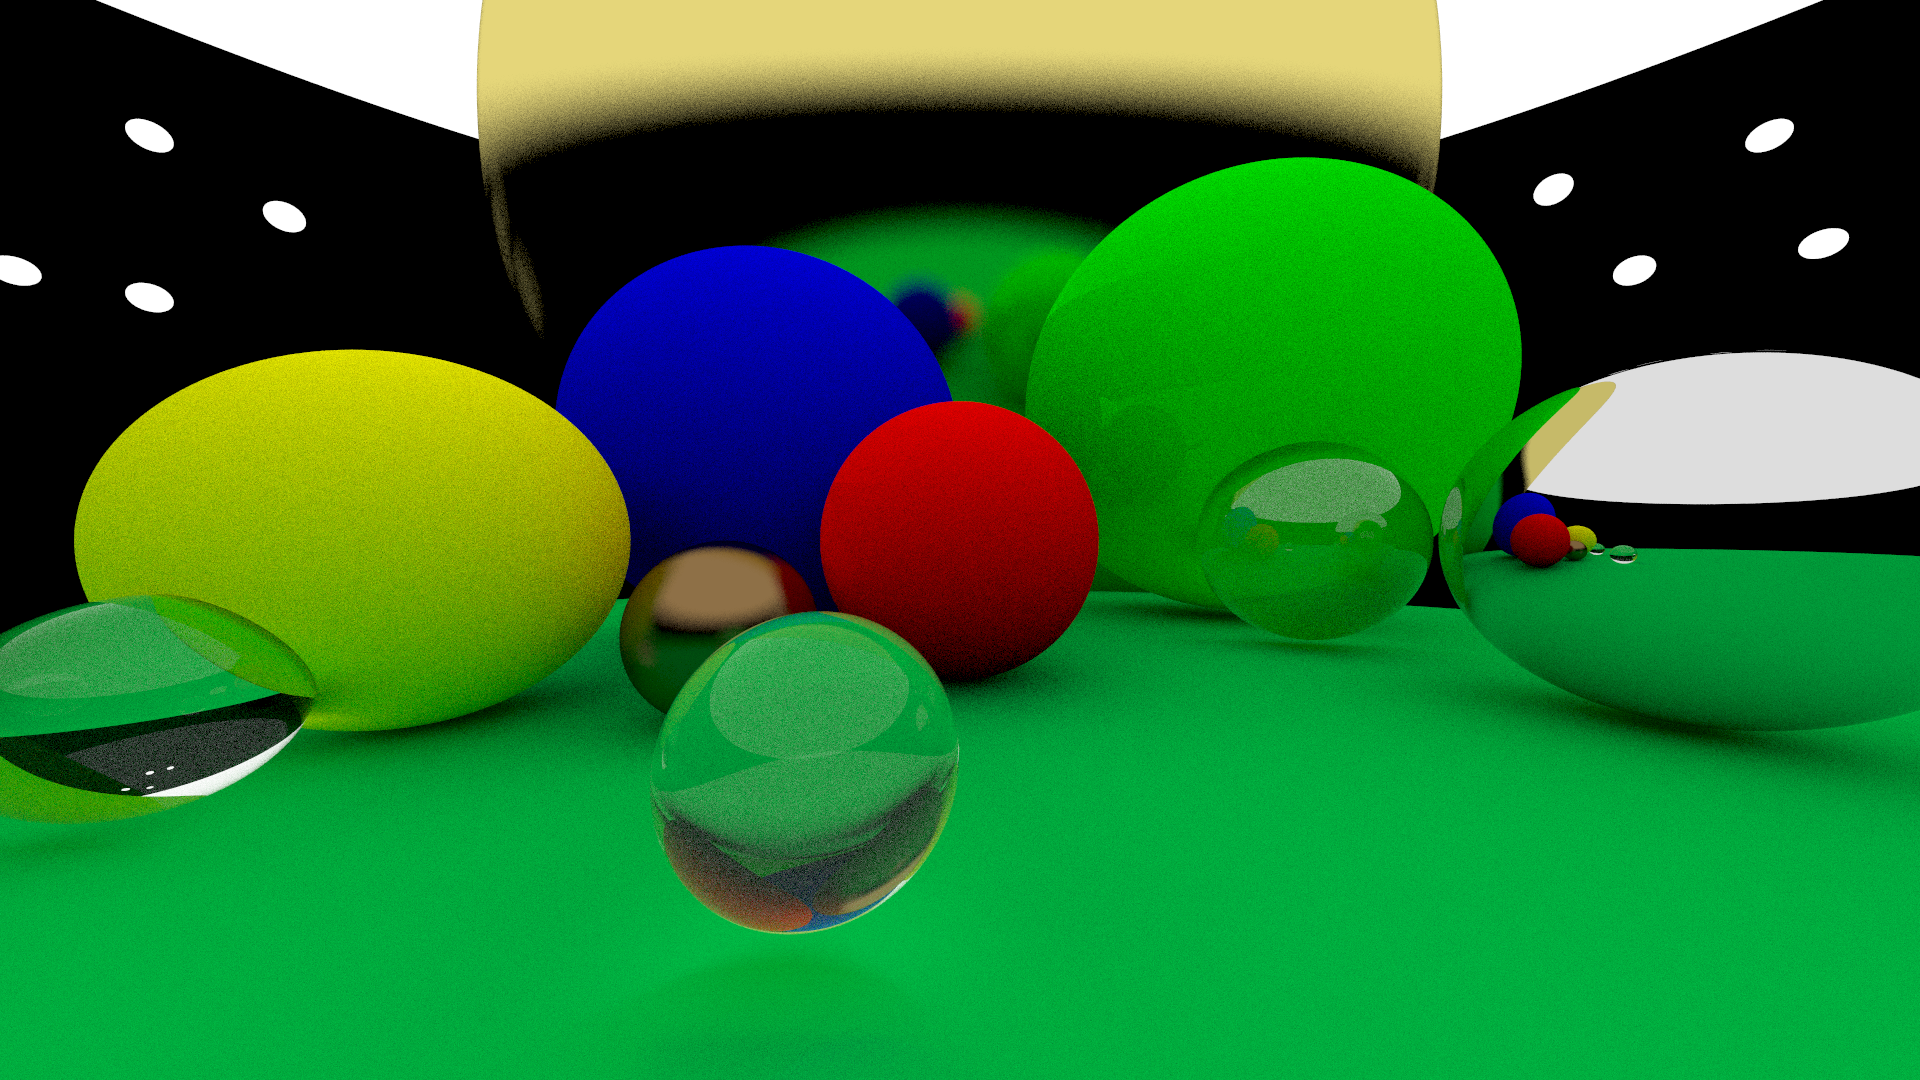
\includegraphics[width=\textwidth]{step8}
\centering
\caption{Image with removed background light but instead light emitting spheres (render depth 16)}
\label{fig:step8}
\end{figure}

\chapter{Positioning and orienting camera}
So far the camera has always been positioned at (0, 0, 0) and looked along the z-axis in the negative direction. This is to be changed so that the camera can be positioned everywhere in the scene and can look in every direction. With this it would be possible to create different images with different point of views from the same scene instead of always having to create an own scene for every image. For that the \textit{Camera} now gets three vectors defining its position:
\begin{itemize}
\item From: Position of the camera
\item At: Where the camera should look at
\item Up: Which way is up, this is used to define the rotation of the camera
\end{itemize}
Using these three parameters, all positions and orientations of the camera are possible. The property definitions of the camera have to be changed to use these three vectors. All changed property definitions are shown in source code \ref{lst:step9}.
\begin{lstlisting}[caption={Updated camera properties}, label=lst:step9, style=mystyle]
self.origin = look_from
self.w = (look_from - look_at).normalize()
self.u = Vector.cross_product(up, self.w).normalize()
self.v = Vector.cross_product(self.w, self.u)
self.horizontal = self.u * self.viewport_width
self.vertical = self.v * self.viewport_height
self.lower_left_corner = (self.origin - self.horizontal / 2 - self.vertical / 2 - self.w)
\end{lstlisting}
An example of different images of the same scene just with different camera positions and orientations can be seen in figure \ref{fig:step9}.
\begin{figure}[h!]
\centering
\begin{subfigure}[h!]{0.475\textwidth}
\centering
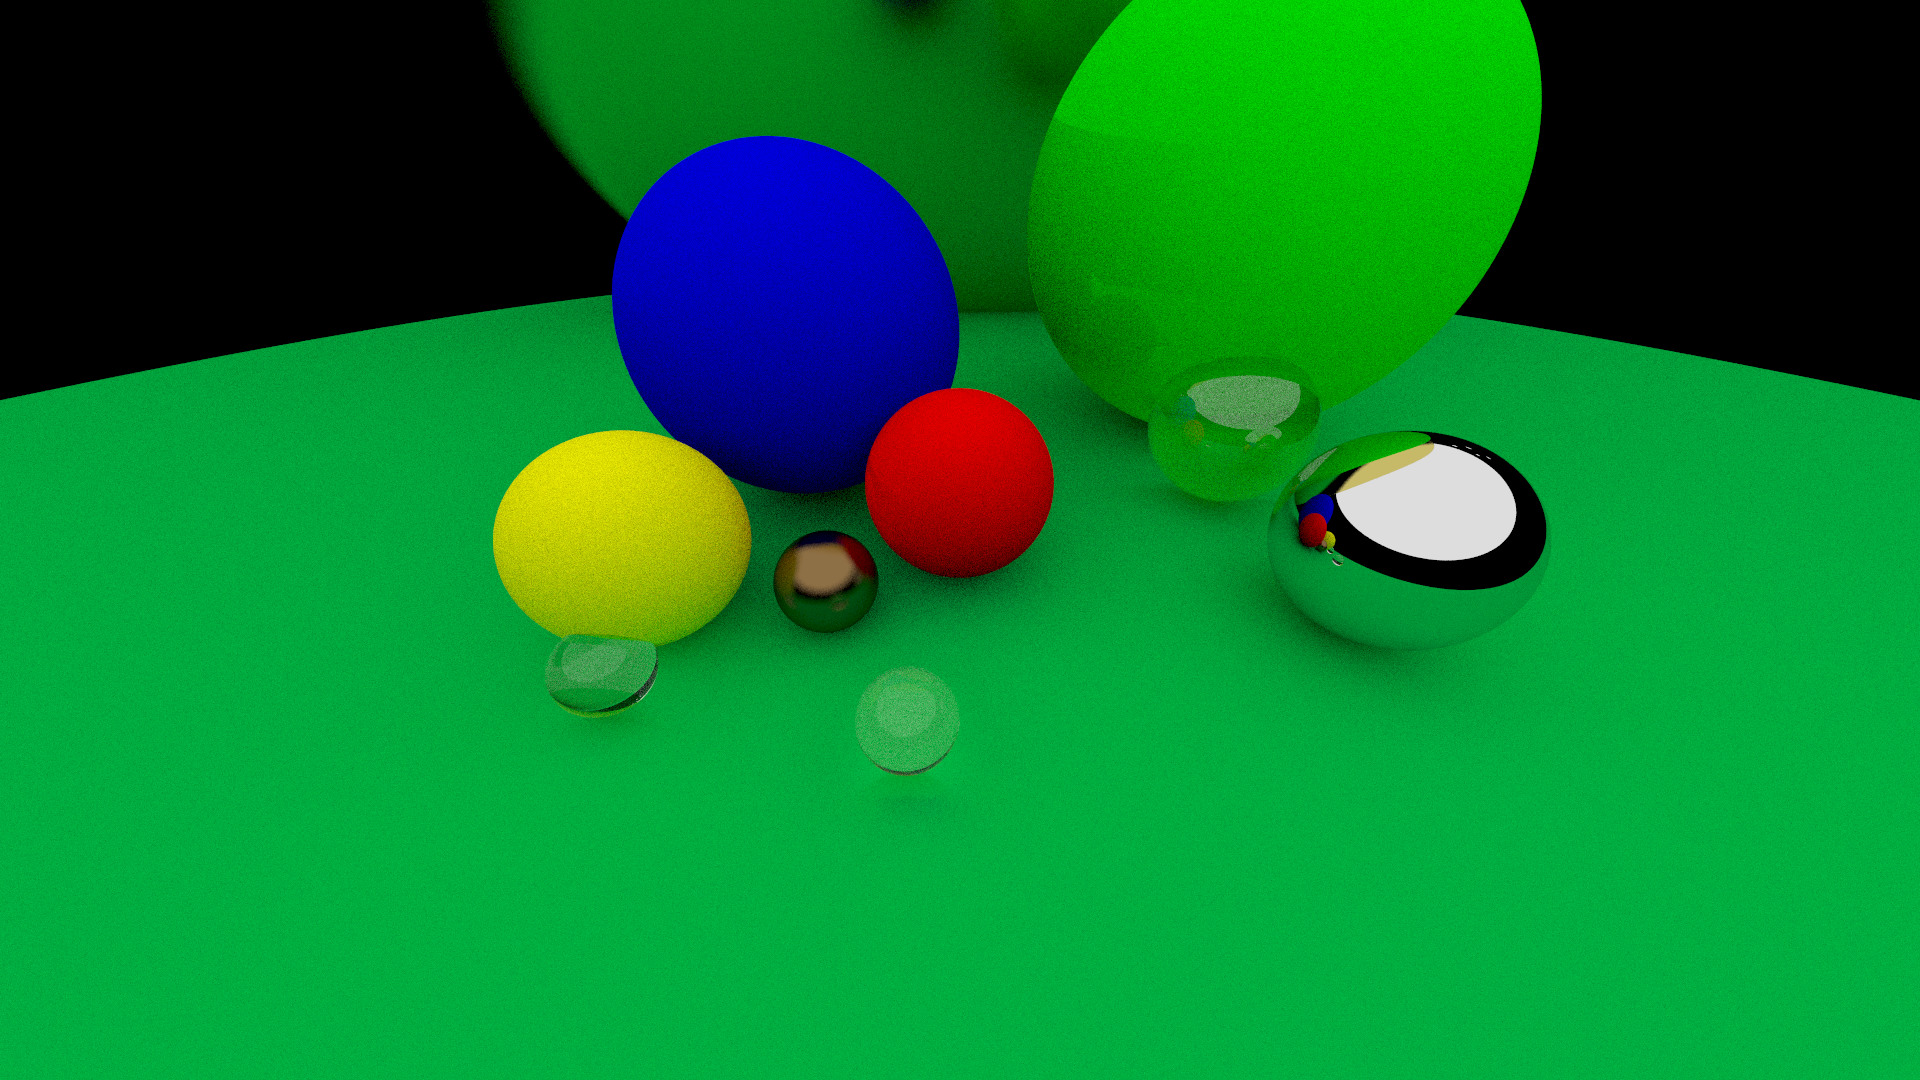
\includegraphics[width=\textwidth]{step9_position1}
\caption{From: (0, 1.5, 0.5)\\At: (0, 0, -1.5)\\Up: (0, 1, 0)}
\end{subfigure}
\hfill
\begin{subfigure}[h!]{0.475\textwidth}
\centering
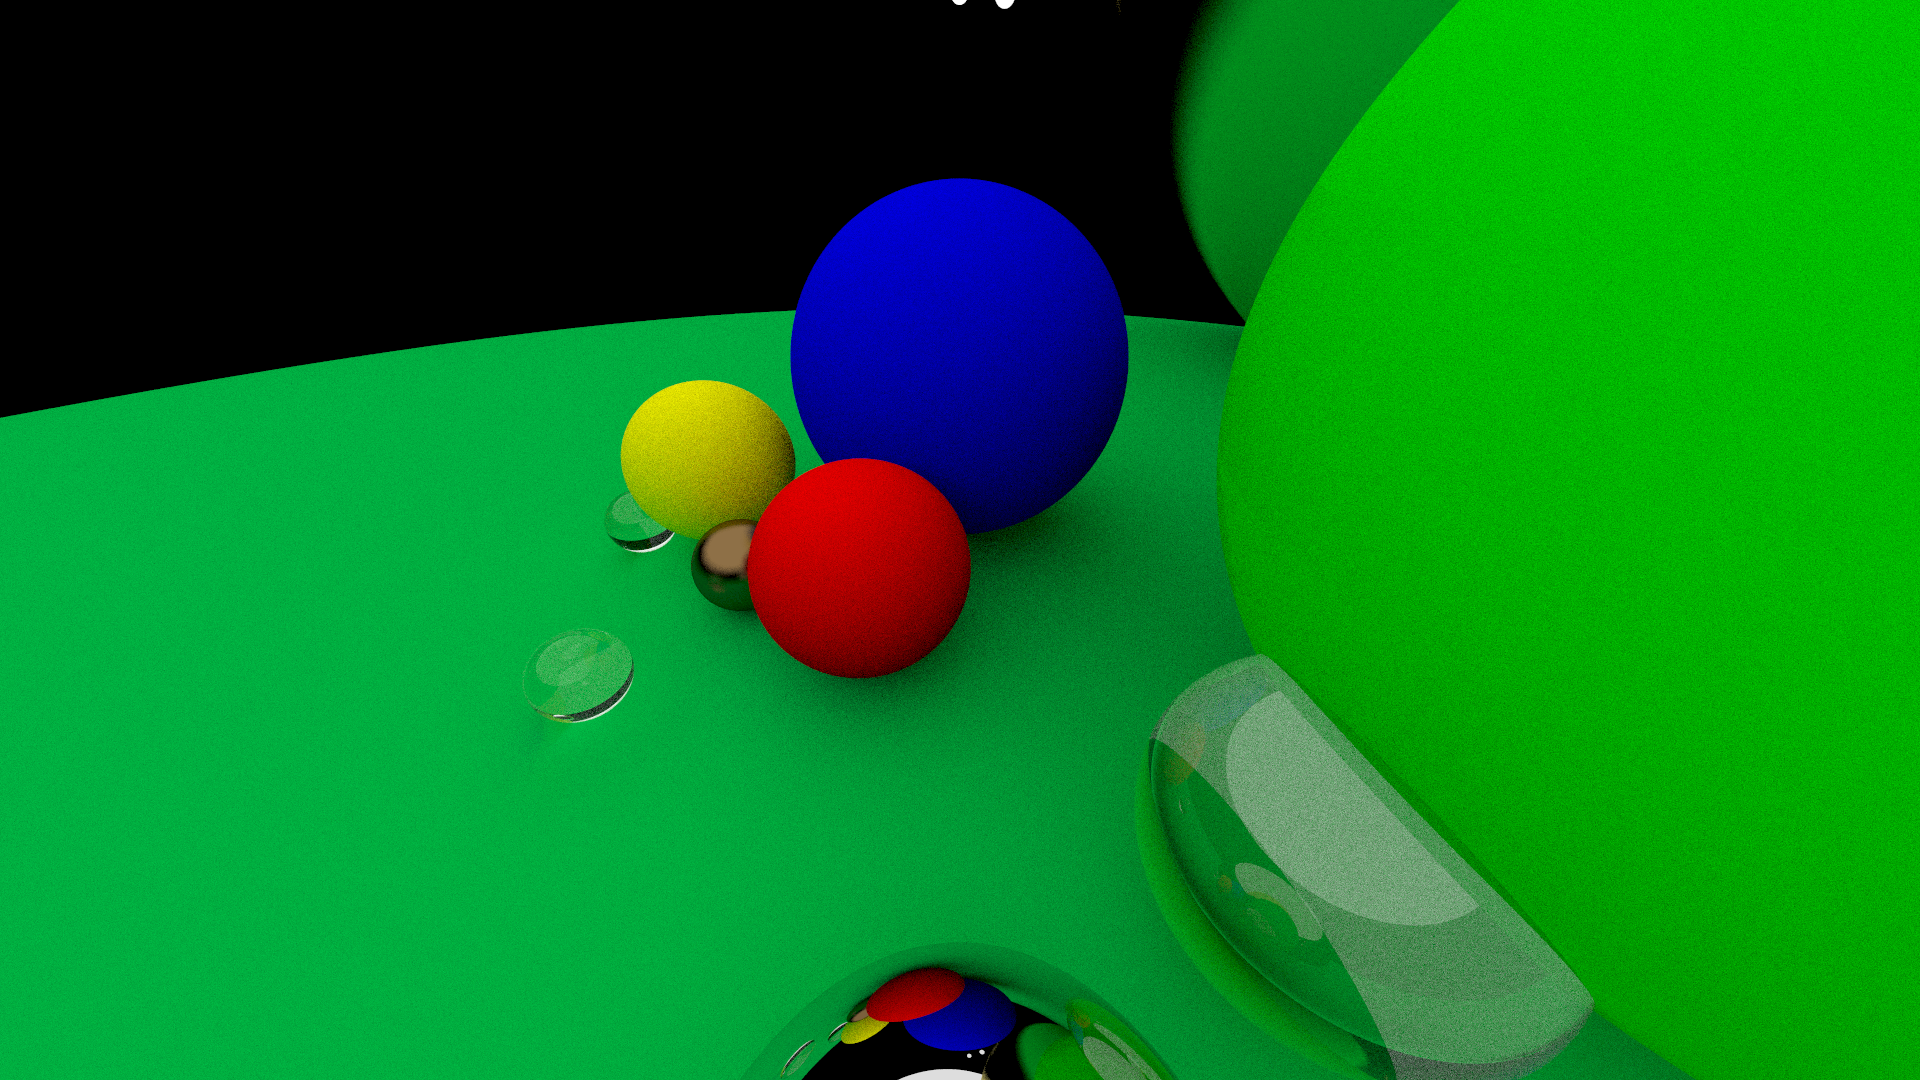
\includegraphics[width=\textwidth]{step9_position2}
\caption{From: (2, 1.5, -1.5)\\At: (0, 0, -2.5)\\Up: (0, 1, 0)}
\end{subfigure}
\vskip\baselineskip
\begin{subfigure}[h!]{0.475\textwidth}
\centering
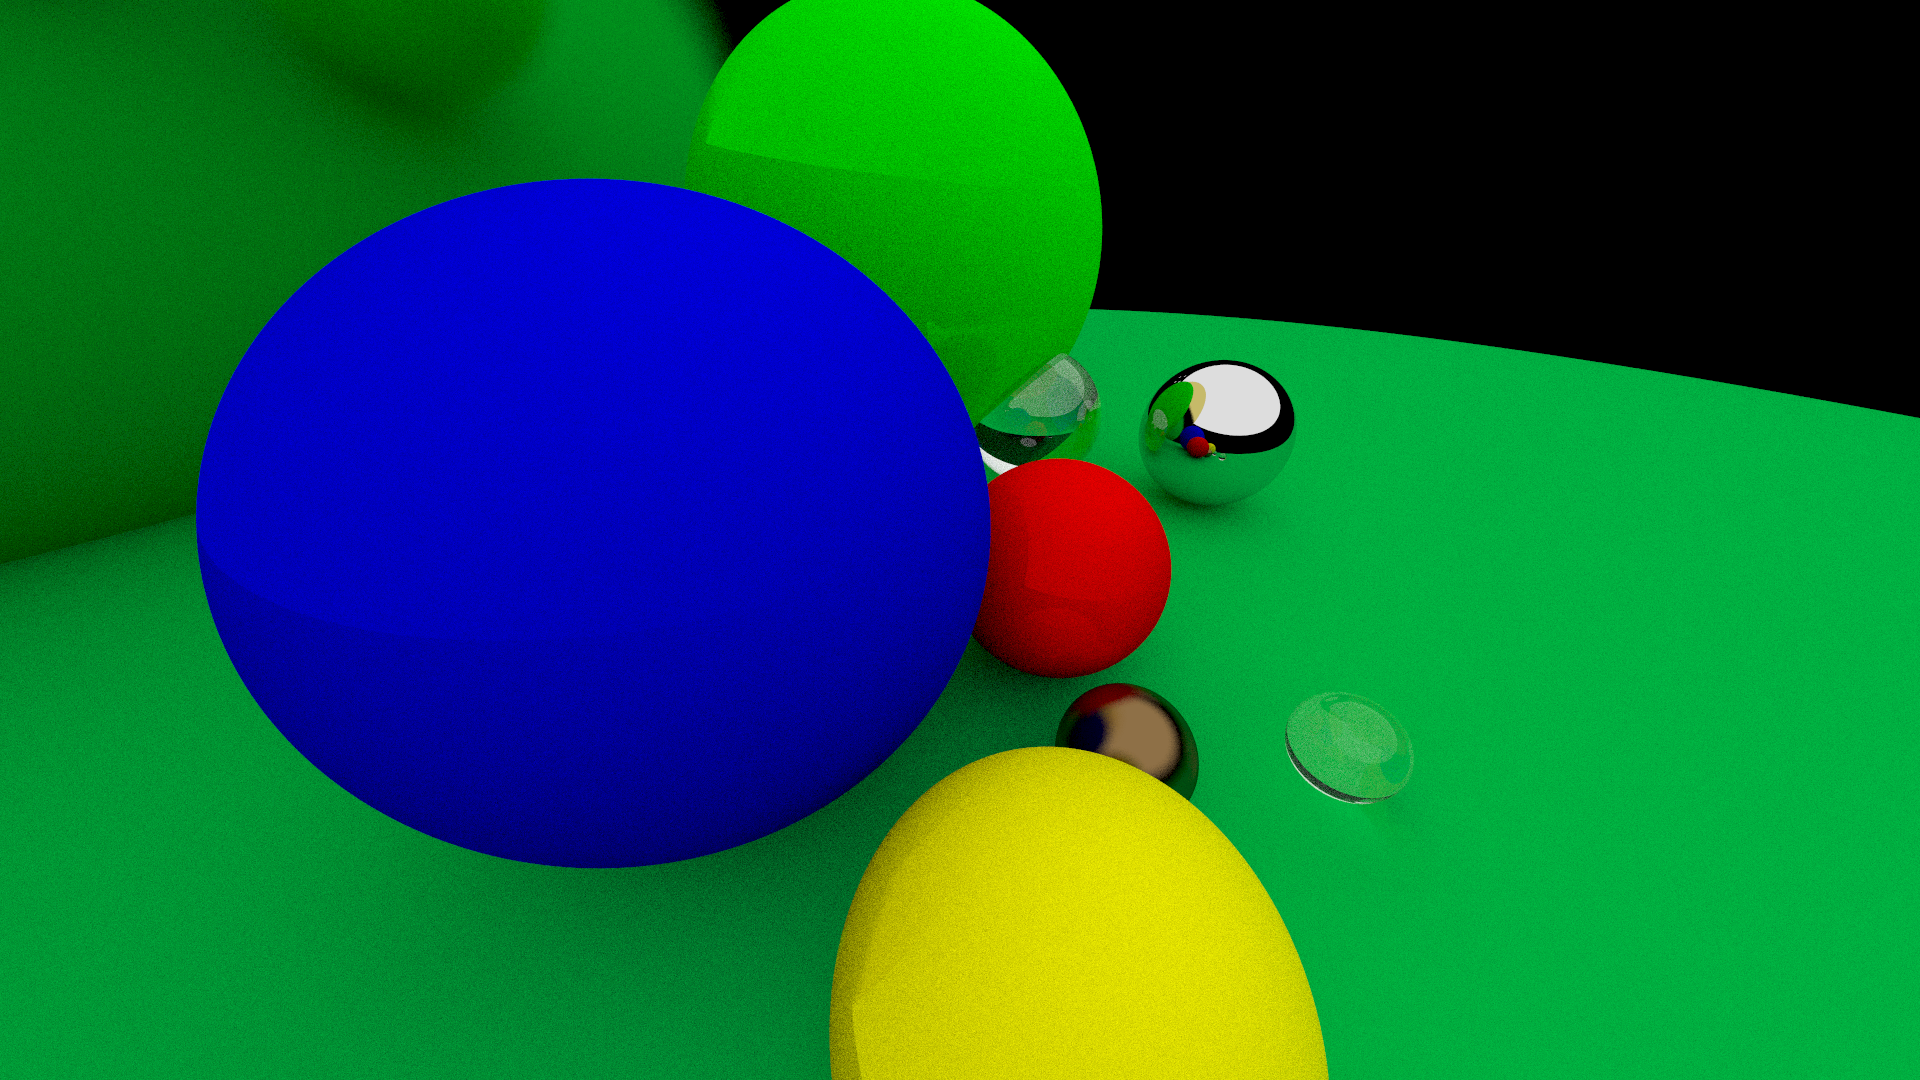
\includegraphics[width=\textwidth]{step9_position3}
\caption{From: (-2, 1.5, -1.5)\\At: (0, 0, -2.5)\\Up: (0, 1, 0)}
\end{subfigure}
\hfill
\begin{subfigure}[h!]{0.475\textwidth}
\centering
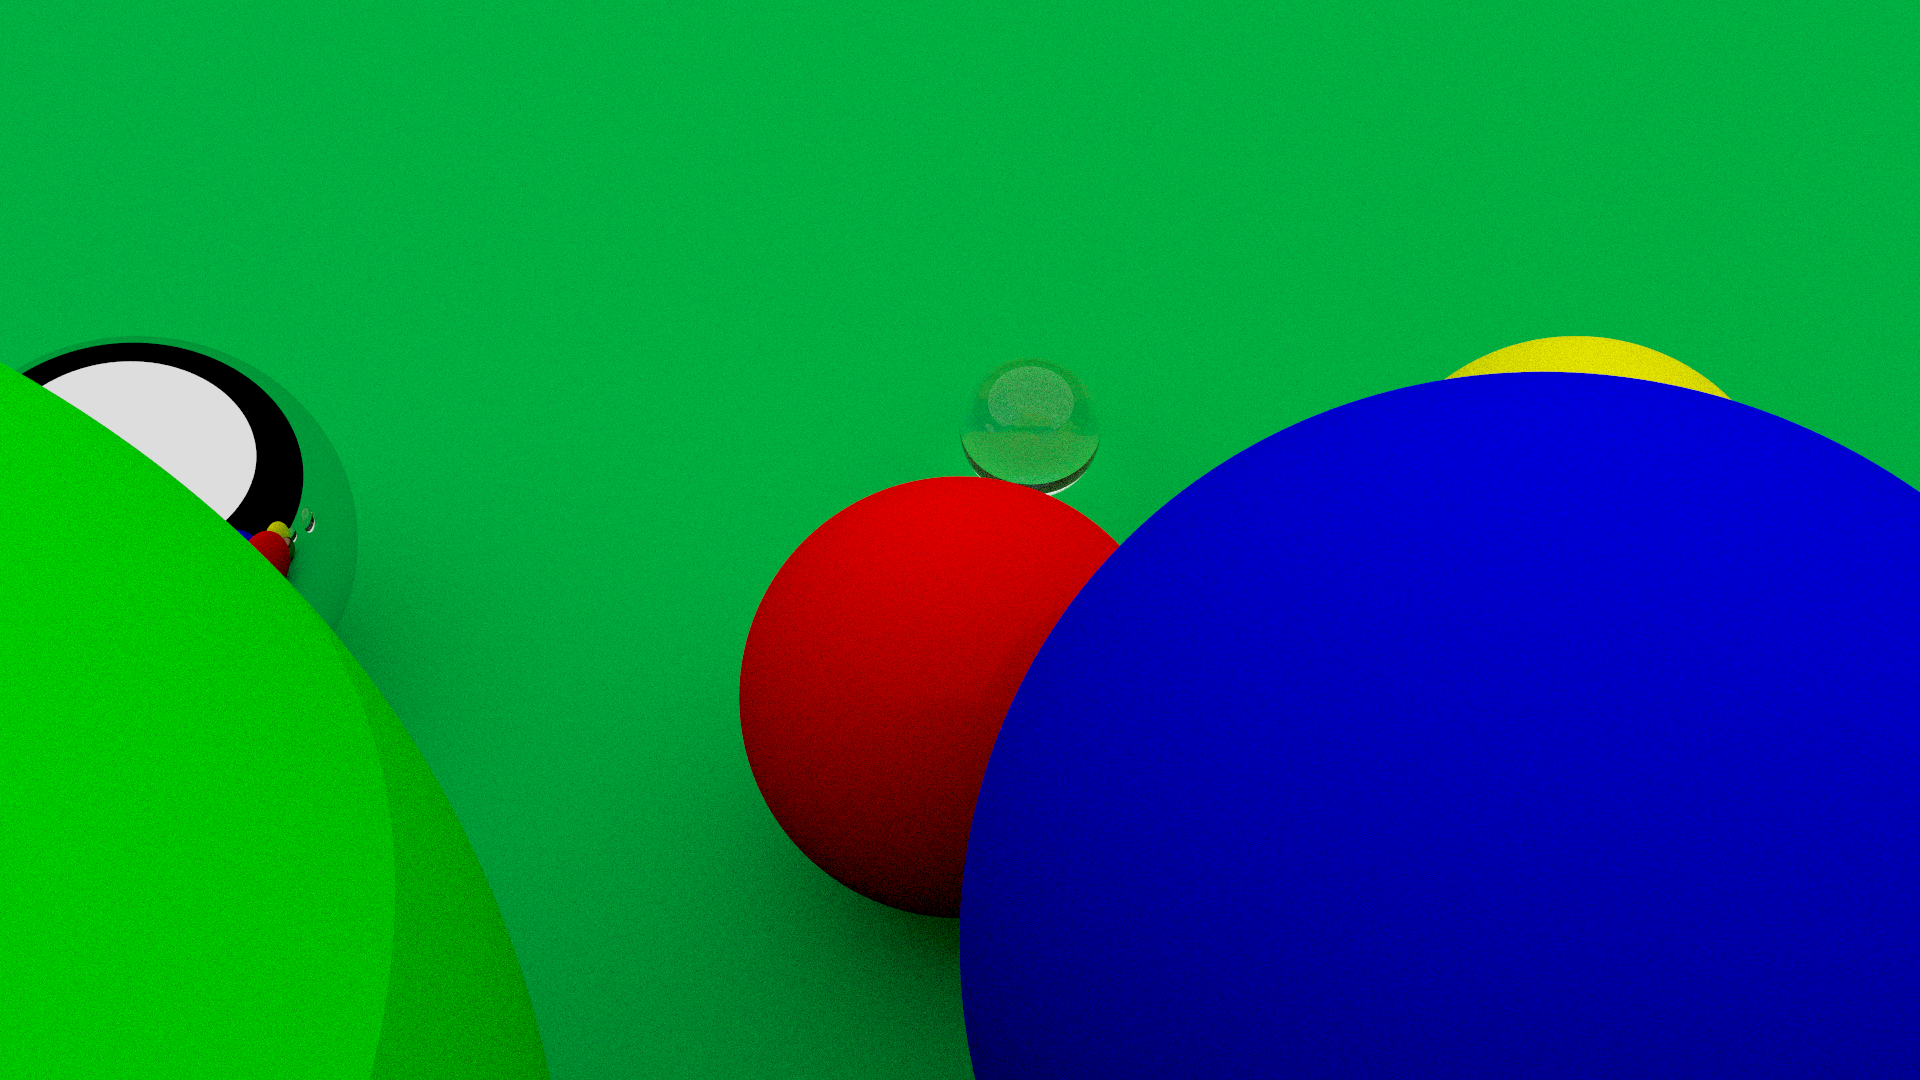
\includegraphics[width=\textwidth]{step9_position4}
\caption{From: (0, 3.5, -5)\\At: (0, 0, -1.5)\\Up: (0, 1, 0)}
\end{subfigure}
\vskip\baselineskip
\begin{subfigure}[h!]{0.475\textwidth}
\centering
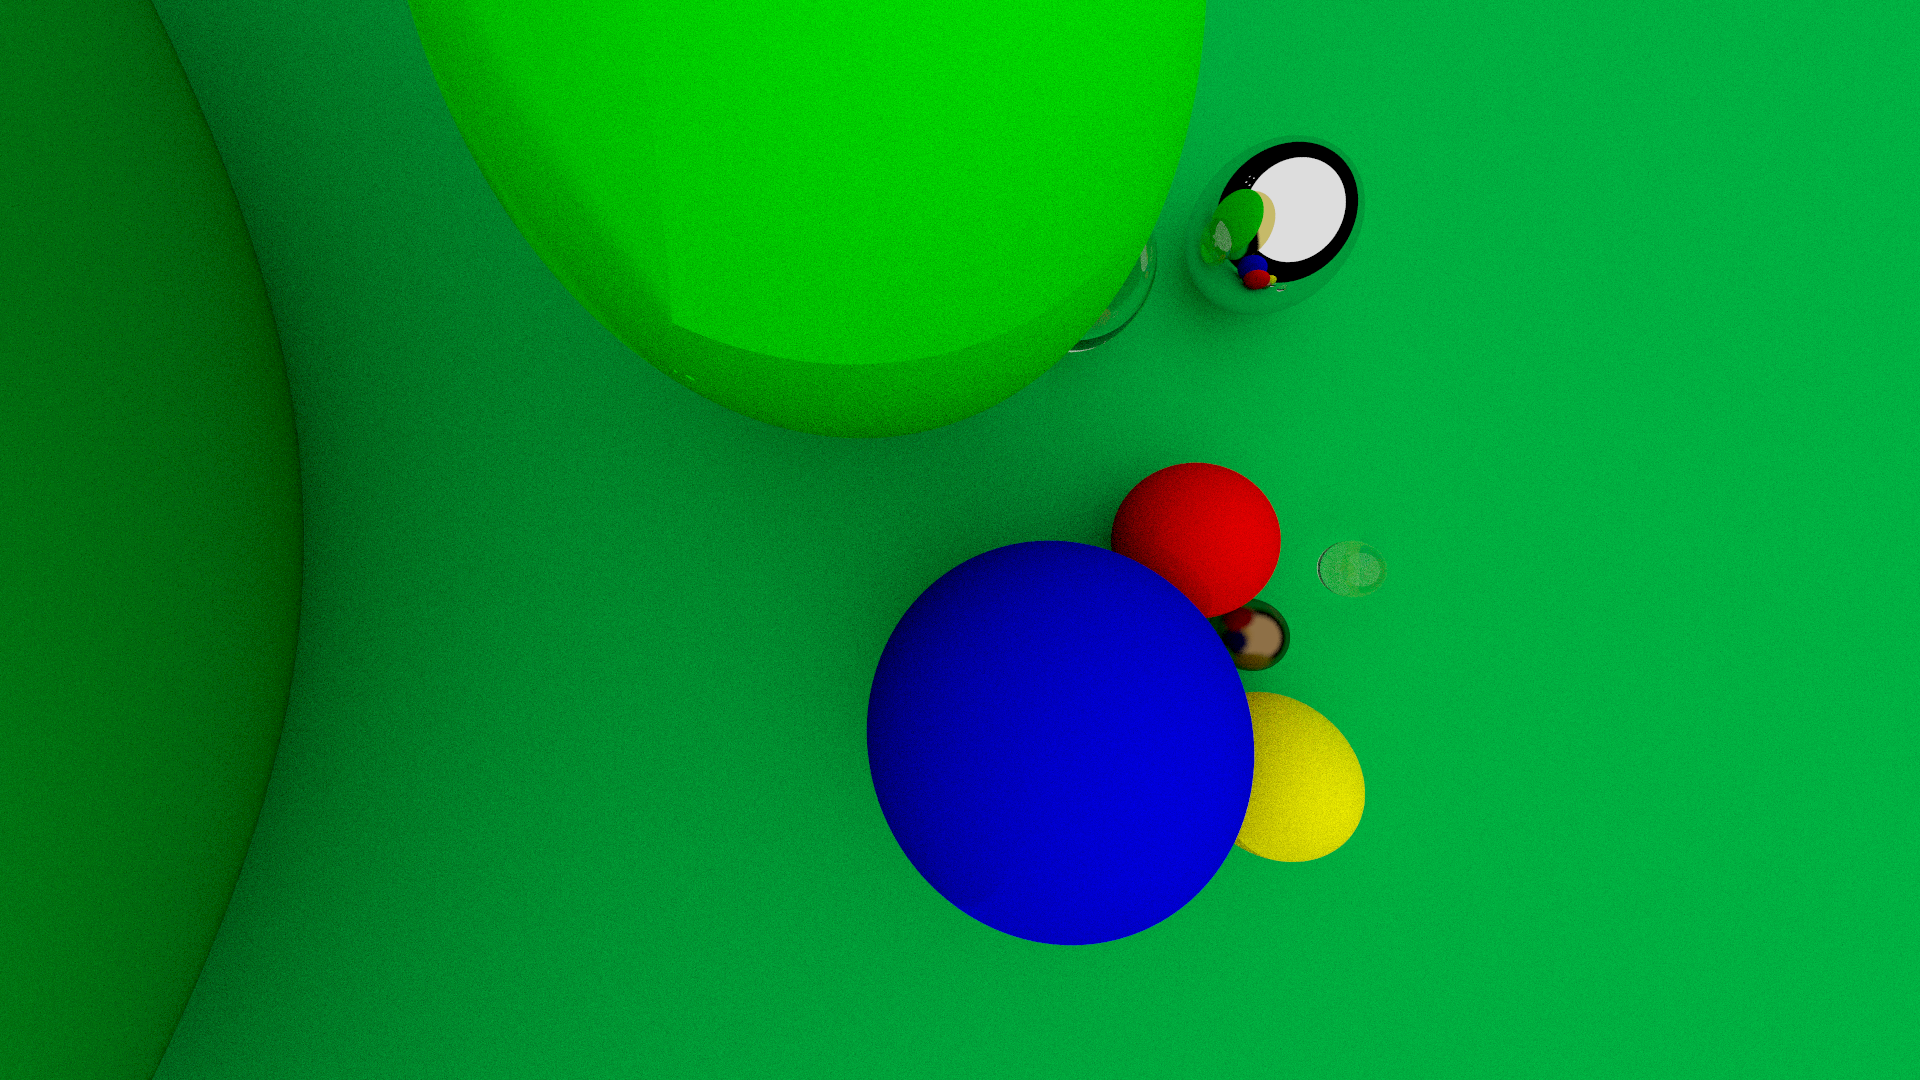
\includegraphics[width=\textwidth]{step9_position5}
\caption{From: (0, 3.5, -3.49)\\At: (0, 0, -3.5)\\Up: (1, 0, 0)}
\end{subfigure}
\caption{Same scene with different camera positions}
\label{fig:step9}
\end{figure}

\chapter{Animation}
All objects in a scene have been static so far, meaning they do not have any movement. To add movement to a scene, the project has to be extended by the concept of time. This means, that the camera and (moving) objects need a time parameter. For the camera this is simply a start time of the image generation and an end time. All rays that are sent out during the rendering process from the camera then simply get a random time of existence in this time interval. For that to be possible, rays also need a time property. This means, that every ray has a time of existence. This time then can be used to get the scene at that moment in time. The spheres not only need a time, but they also need information about their movement. Therefore, \textit{Sphere} objects can now accept a destination, start time of their movement and a time when they reach their destination. The movement of the spheres is assumed to be linear and starting at its origin at the start time going to the destination where they arrive at the end time. It is furthermore assumed, that after the end time and before the start time the sphere moves in the same way as in that interval and thus the position can easily be computed by a linear equation. The implementation of this is shown in source code \ref{lst:move}.
\begin{lstlisting}[caption={Computing position of sphere}, label=lst:move, style=mystyle]
def move(self, time: float | None) -> Vector:
    if self.movement is None or time is None:
        return self.origin
        
    target, time0, time1 = self.movement
    return self.origin + (target - self.origin) * ((time - time0) / (time1 - time0))
\end{lstlisting}
This now has to be used as the position of a sphere when testing if a ray hits the sphere. As with previous extensions of the project, it is important to still be able to reproduce previous images. To achieve this, the time and movement information is made optional and if a sphere does not have movement, the function simply returns its origin. The same goes for the camera and rays, for both a time component is optional. Because now a moving object is represented by a static image, motion blur occurs. This simply means, that the object seems to be at multiply positions at the same time. This can be seen in figure \ref{fig:step10}, where one of the ''stars'' in the background now has movement as well as the glass ball in the foreground and the green sphere.
\begin{figure}[h!]
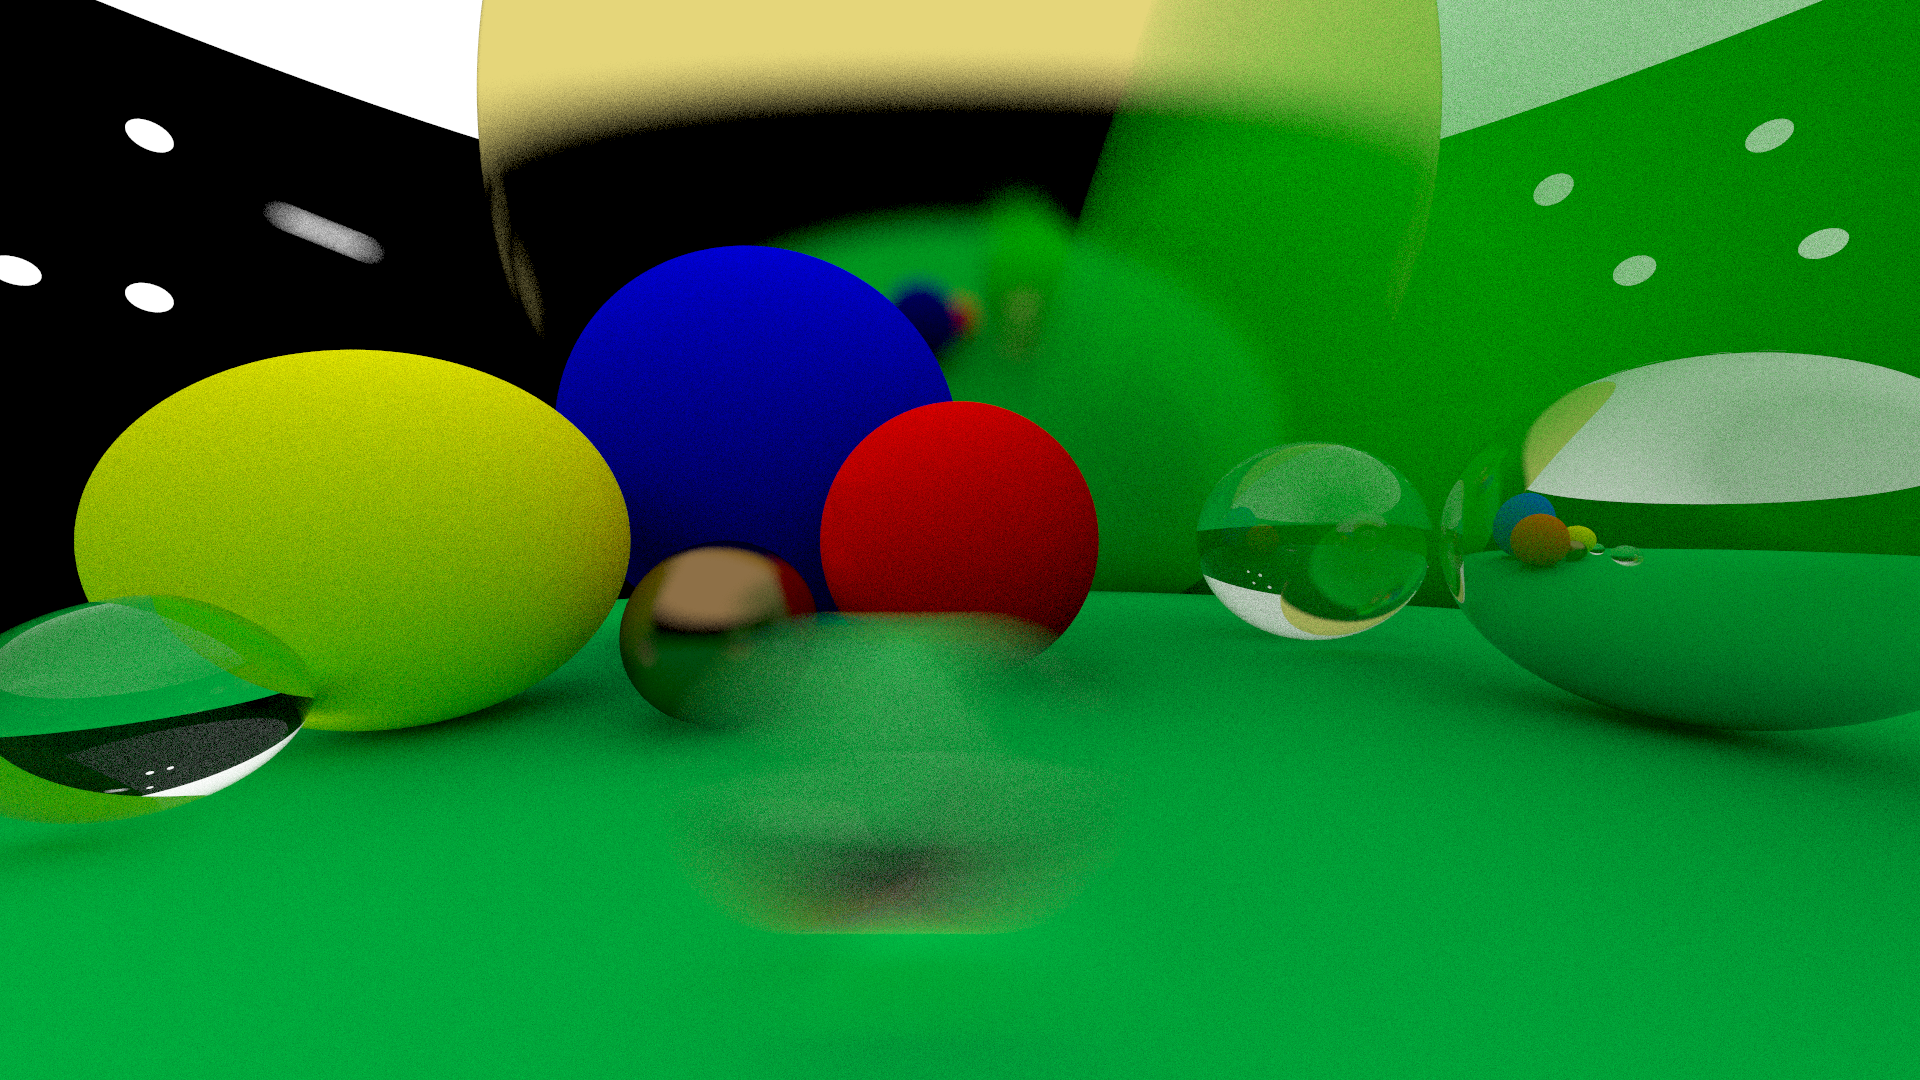
\includegraphics[width=\textwidth]{step10}
\centering
\caption{Motion blur caused by moving objects}
\label{fig:step10}
\end{figure}

\chapter{Render parallelization}
The rendering process with a higher image quality takes quite a long time. To make the rendering faster, it shall be run in parallel on multiple cores on the CPU. Because the computation of the color of a pixel is independent of the color of other pixels, the image can simply be split into multiple smaller images. Every of these image parts can then be rendered independently and on multiple cores. It is chosen to split the image horizontal into as many stripes as cores should be used. This is done because the spheres should be more equally distributed over the cores this way and the spheres are what take most of the computation time. To render only a specific area of rows instead of the whole image, a new render function is added to the \textit{Camera}. This takes the additional information at which row it should start and till which row it should render. Because it is not that easily possible to return an \textit{Image} object from a different core to the ''main'' process, a different way of saving the results has to be chosen. The simplest and memory efficient form is using an array. This can be created for the whole image and shared between all processes and cores and thus the smaller parts do not have to be assembled at the end. Every process just writes into the part it renders and because of that an array without access control can be used, which (slightly) improves the performance. Hence, the rendering function additionally takes also the array for its results. For a better parameter handling, a class for the processes is created (\textit{RenderingProcess}), which takes all for the rendering required parameters and starts a new process on a different core for rendering an image part. Additionally, the render method of the \textit{Scene} has also to be adopted to use the new parallelized rendering process. This is shown in source code \ref{lst:parallel}. Because the results are an array, they have to be converted to an \textit{Image} object. To optimize this, the \textit{Image} is changed to accept an array as input and then use this array as the internal representation of the image, using it for all functions. This removes the necessity to iterate through the whole array just to convert it into a two-dimensional list. After converting the result into an image, the same interface for the parallelized and serial rendering process are created. This means, that they can be used interchangeably depending on the current requirements.
\newpage
\begin{lstlisting}[caption={Parallelizing the rendering process}, label=lst:parallel, style=mystyle]
def render(self, width: int, render_depth: int, in_parallel: bool = True, number_cores: int = 0) -> Image:
    if not in_parallel:
        return self.camera.render(width, render_depth, self.world, self.background)

    max_cores = mp.cpu_count()
    if not 0 < number_cores <= max_cores:
        number_cores = max_cores

    processes = []
    
    height = int(width // self.camera.aspect_ratio)
    rows_per_process = int(height // number_cores)
    
    results = mp.RawArray('B', height * width * 3)
    
    for i in range(number_cores - 1):
        process = RenderingProcess(width, render_depth, self.world, i * rows_per_process, (i + 1) * rows_per_process, self.camera, results, self.background)
        processes.append(process)
        process.start()

    height_start = (number_cores - 1) * rows_per_process
    self.camera.render_parallel(width, render_depth, self.world, height_start, height, results, self.background)
    
    for process in processes:
       process.join()

    return Image(width, height, array=results)
\end{lstlisting}
\newpage
\noindent To see if the parallelization achieved significant improvements, a comparison of the rendering time is done. For that, the same scene is rendered multiple times using a different number of cores. The results of that comparison is shown in figure \ref{fig:efficiency}.
\begin{figure}[h!]
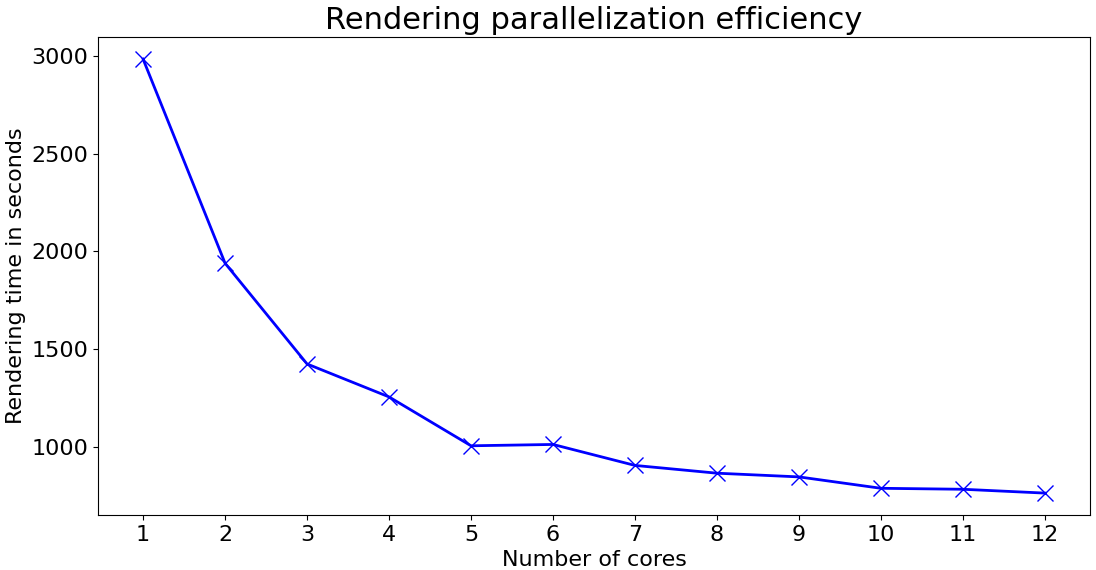
\includegraphics[width=\textwidth]{parallelization_efficiency}
\centering
\caption{Comparison of parallelization efficiency with a different number of cores}
\label{fig:efficiency}
\end{figure} \\
From the graph can be seen, that the more cores are used for the rendering the faster the rendering is done. The speedup (figure \ref{fig:speedup}) shows, that by using the parallelization a big improvement is achieved. Using 12 cores, the rendering is almost four times as fast. By using the parallelization, an image can be rendered with a for times higher resolution in the same time (e.g. 4K can be rendered on 12 cores in the same time as a Full HD image on one core). An even better speedup will most likely be achieved using more cores. Because most CPUs only have a strongly limited number of cores, using an GPU for the parallelization would yield even better results. This would be an interesting next step for the further development of the parallelization.
\begin{figure}[h!]
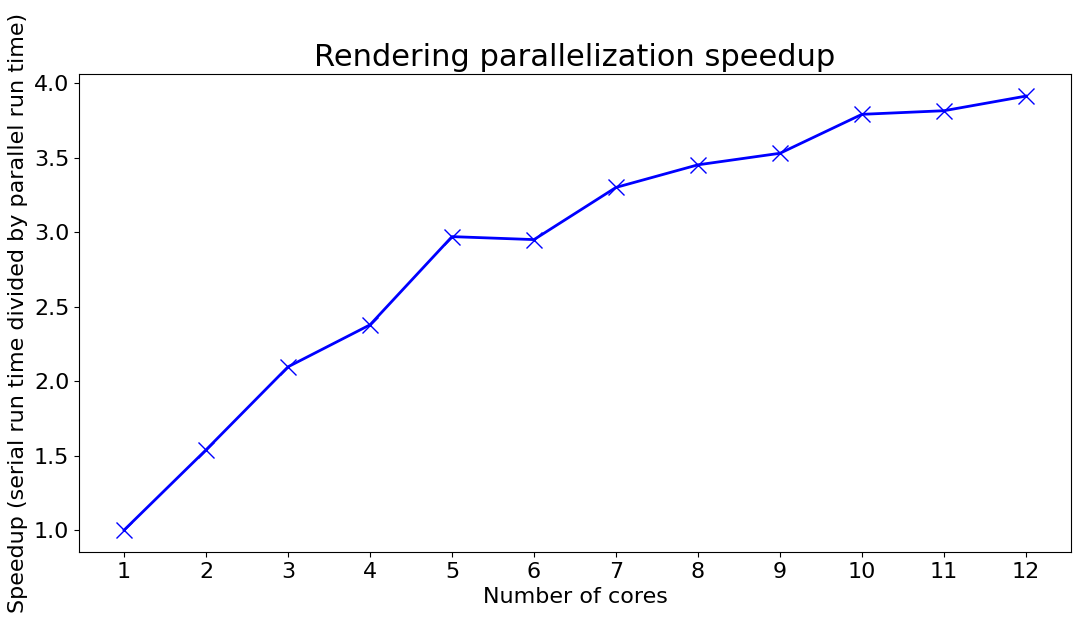
\includegraphics[width=\textwidth]{parallelization_speedup}
\centering
\caption{Achieved speedup by rendering parallelization}
\label{fig:speedup}
\end{figure}

\chapter{Config files}
To not always having to change the code and render multiple images automatically, config files should be used. These config files are used as a description of the scene and the parameters needed for rendering. A config file then needs to be converted into a scene that can be rendered. The creation of a scene from a config file is done by the script \textit{run}. It takes the path to a config file, creates a scene from it and renders the scene using the parameters also from the config file. As format of the config files JSON is chosen, because it has an easy and simple syntax and can easily be read by a Python library. JSON uses simply data-structures similar to Python such as dictionaries or lists. This makes accessing data from a JSON file in Python effortless. An example of a config file is shown in source code \ref{lst:config}.
\begin{lstlisting}[caption={Config file example}, label=lst:config, language=json]
{"background": [0, 0, 0],
"camera": {
	"look_from": [0, 0, 0],
	"look_at": [0, 0, -1],
	"up": [0, 1, 0],
	"vfov": 90,
	"focal_length": 1,
	"aspect_ratio": 1.7777777777777777777777777777777777777777777777777777777777777777777777777777777777777777778,
	"viewport_height": 2,
	"samples_per_pixel": 32
	},
"rendering": {
	"width": 1080,
	"render_depth": 32,
	"in_parallel": true,
	"number_cores" : 0
	},
"saving": {
	"path": "results/test.ppm",
	"gamma_correct": true
	},
"spheres": [{
	"origin": [-2, 1, -4],
	"radius": 2,
	"material": {
			"type": "emissive",
			"color": [100, 150, 200],
			"intensity": 0.75
			},
	"movement": [[-3, 1, -2], 0, 1]
	},
	{
	"origin": [-2, 1, -2],
	"radius": 1,
	"material": {
			"type": "transmissive",
			"color": [255, 255, 255],
			"refraction_index": 1.5
			},
	"movement": [[-3, 1, -2], 0, 1]
	}]
}
\end{lstlisting}

\end{document}